\documentclass[letterpaper,11pt]{article}

\usepackage[margin=1in]{geometry}
\setlength\parindent{0pt}
\setlength{\parskip}{0.7em}

\usepackage{titlesec}
\titlespacing*{\section}{0pt}{0.6\baselineskip}{0.2\baselineskip}
\titlespacing*{\subsection}{0pt}{0.4\baselineskip}{0.1\baselineskip}
\titlespacing*{\subsubsection}{0pt}{0.3\baselineskip}{0.1\baselineskip}

\usepackage{enumitem}
\setlist{nosep, topsep=2pt}

\usepackage{graphicx}
\usepackage{subcaption}
\usepackage{booktabs}
\usepackage{multirow}
\usepackage{amsmath}
\usepackage{amssymb}
\usepackage{float}
\usepackage{bm}
\usepackage[hidelinks]{hyperref}

% docmute strips \documentclass/\begin{document}/\end{document} from \input files
\usepackage{docmute}

\title{Lab 3 Report: Connecting Language to fMRI\\
       }
\author{}
\date{}

\begin{document}
\maketitle

\section{Introduction}

Understanding how the brain processes language is one of the central questions in cognitive neuroscience. When we listen to a story, different regions of the brain respond in distinct ways, some track sounds, others track meaning, and others integrate information across sentences. Functional MRI (fMRI) lets us measure these responses at the level of individual voxels, small cubic regions of brain tissue, by recording changes in blood-oxygen levels (BOLD signal) as a subject listens. If we can build a model that accurately predicts these voxel responses from the text of what someone heard, it can help to understand how the brain processes language.


This lab tackles exactly that problem. We work with data from two subjects (\textit{s2} and \textit{s3}) collected by the Huth Lab at UT Austin \cite{jain2018incorporating}, who each listened to a set of podcast stories while lying in an fMRI scanner. The goal is to learn a mapping from the words in each story to the corresponding brain responses, using text embeddings as input features and ridge regression as the model. The core question is how much the choice of embedding matters: does it make a difference whether we represent words as simple counts, as dense semantic vectors, or as context-sensitive representations from a large language model?


We evaluate several embedding configurations of increasing sophistication across five families---Bag-of-Words (BoW), Word2Vec, GloVe, and BERT-based variants, and LoRA fine-tuned configurations differing in training recipe and extraction layers---and ask whether different methods predict the same voxels, where the gains from contextual models are concentrated, and what individual words drive predictions in the best-performing voxels using SHAP and LIME.

\section{Data}
\label{sec:data}
\subsection{fMRI and Text Data}
\label{sec:data-fmri}

The data come from the Huth Lab at UT Austin \cite{jain2018incorporating} and consist of whole-brain BOLD fMRI recordings from two subjects (\textit{s2} and \textit{s3}) listening to 101 naturalistic podcast stories.  BOLD responses were acquired at a repetition time of $\text{TR} = 2$\,s, yielding 256 raw volumes per story.  Subject~\textit{s2} has 94{,}251 cortical voxels and subject~\textit{s3} has 95{,}556 voxels.

For each subject--story pair, the fMRI signal is a matrix $\bm{Y} \in \mathbb{R}^{T \times V}$, where $T$ is the number of usable scan timepoints per story (after trimming scanner equilibration and the post-stimulus BOLD tail, detailed in Section~\ref{sec:ridge}) and $V$ is the number of cortical voxels.  Alongside the fMRI data, we have word-level transcripts with precise onset timestamps, which are used to align each word's text embedding to the TR time grid.

Stories were divided at the story level into 81 training stories and 20 test stories.  All models are fitted exclusively on training stories and evaluated on the held-out test stories, keeping the two splits completely separate throughout.


\graphicspath{{results/regression/}}
\graphicspath{{../results/figures/regression_analysis/}}
\maketitle


\section{Method}


We build voxelwise brain encoding models that predict BOLD fMRI responses from
the text of naturalistic audio stories.  Eight embedding configurations across
five families are evaluated---from a non-semantic bag-of-words baseline to a
LoRA fine-tuned BERT model reading from middle transformer layers---all fitted
via ridge regression with efficient SVD-based per-voxel regularization selection.



Words are produced at an irregular rate (${\sim}2$--4\,words/s), whereas fMRI
samples uniformly at 0.5\,Hz.  The following three operations, applied
identically across all representation methods, bring both signals onto a common
time grid and account for the sluggish hemodynamic response.


\subsection{Preprocessing}
Let $\bm{E} \in \mathbb{R}^{N \times d}$ denote the word-rate embedding matrix
for a story with $N$ words and embedding dimension $d$.  We resample $\bm{E}$ to
the TR grid using Lanczos sinc interpolation, leveraging the per-word onset
timestamps stored in the dataset, yielding
$\bm{E}_{\mathrm{TR}} \in \mathbb{R}^{256 \times d}$.  Lanczos interpolation
preserves spectral content to a greater degree than nearest-neighbor or linear
resampling, which matters because the BOLD signal occupies a narrow low-frequency
band.



We discard the first 5 TRs (10\,s) to remove scanner equilibration artifacts and
the final 10 TRs (20\,s) to avoid the residual BOLD tail extending past the audio
stimulus, yielding $T = 241$ timepoints per story.  The fMRI response matrices
$\bm{Y}$ are pre-trimmed identically during dataset preparation; no further
trimming is applied to $\bm{Y}$.



The BOLD signal lags neural activity by approximately 4--6\,s.  Rather than
convolving with a fixed hemodynamic response function (HRF), we model the HRF
implicitly by stacking four time-shifted copies of
$\bm{E}_{\mathrm{TR}}[6{:}-10, :]$ (post-trim) at delays
$\delta \in \{1, 2, 3, 4\}$\,TRs:
%
\begin{equation}
  \bm{X} = \bigl[\bm{E}^{(\delta=1)},\; \bm{E}^{(\delta=2)},\;
                  \bm{E}^{(\delta=3)},\; \bm{E}^{(\delta=4)}\bigr]
  \;\in\; \mathbb{R}^{T \times 4d}.
\end{equation}
%
This quadruples the feature dimension and allows the ridge model to learn a
per-voxel hemodynamic filter from data.  Stacking training stories gives
$\bm{X}_{\mathrm{train}} \in \mathbb{R}^{27678 \times 4d}$ and
$\bm{X}_{\mathrm{test}} \in \mathbb{R}^{7108 \times 4d}$.


\subsection{Text Representations}


We compare six text representation methods spanning a broad range of semantic
and contextual richness.
\subsubsection{Baseline Embeddings}
We used three major textual embeddings for baseline analysis, including 

(1)Bag of Words: A \texttt{CountVectorizer} is fit on the union of all training and test stories
to build a vocabulary of ${\approx}12{,}000$ types.  Each word is encoded as a
one-hot sparse vector; after delay stacking the feature dimension is
$4 \times 12{,}000 \approx 48{,}000$.  Because the BoW matrix is
${\sim}99.99\%$ sparse, a dedicated sparse solver is used (Section
\ref{sec:sparse_solver}).



(2) Word2Vec: We use the Google News skip-gram model pretrained on ${\sim}10^{11}$ tokens,
which provides 300-dimensional dense vectors per word.  Out-of-vocabulary words
are mapped to zero vectors.  Final dimensionality: $4 \times 300 = 1{,}200$.



(3) Glove: We use the Stanford 840B Common Crawl GloVe vectors (300-d); lookup is
case-insensitive.  Out-of-vocabulary words are zeroed.  Final dimensionality:
$4 \times 300 = 1{,}200$.

\subsubsection{Contextual Representations with BERT}

We extract contextual word embeddings from \texttt{bert-base-uncased} (12
transformer layers, hidden size $d_h = 768$, 110M parameters).  WordPiece
subword tokens are pooled to one vector per original word by averaging over
subword token positions.  All four BERT-based methods share this tokenization
and pooling step; they differ in (a) how much surrounding context each word
receives, (b) which transformer layers are read out, and (c) whether the
model weights have been fine-tuned on podcast text.


(1) Baseline (reference) BERT: As a reference, each story is split into non-overlapping 128-word chunks that
are fed independently to BERT.  The final layer's hidden state
($\ell = 12$) is used directly.  Words at chunk boundaries receive no context
from adjacent chunks.  Final dimensionality: $4 \times 768 = 3{,}072$.



(2) Enhanced BERT: We apply two modifications over the vanilla baseline to improve the quality of
the contextual signal passed to the ridge model.

\textbf{Sliding-window context.}
Stories are processed with overlapping windows of 256 words and a stride of 128
words (50\% overlap), safely within BERT's 512-token limit
(${\sim}1.3$ tokens/word on average).  Each word appears in up to two windows;
its embeddings are averaged across windows, giving boundary words access to
richer bilateral context and eliminating the context-truncation artifacts of
independent chunking.

\textbf{Multi-layer averaging.}
We average the hidden states of the last four transformer layers
($\ell \in \{9,10,11,12\}$) rather than using only the final layer.  This
\texttt{last4\_mean} strategy blends high-level semantic content captured in the
upper layers with structural and syntactic information retained in lower layers,
and is widely reported to improve downstream representation quality.

Final dimensionality: $4 \times 768 = 3{,}072$.

\subsubsection{Domain Adaptation via LoRA Fine-Tuning}
\label{sec:lora}



(1) LoRA Training Setup (shared across all LoRA variants): To adapt BERT to the podcast domain, we fine-tune \texttt{bert-base-uncased} on
the 81 training stories using Low-Rank Adaptation (LoRA; Hu et al., 2022) with
a masked language modeling (MLM) objective.  LoRA injects trainable rank-$r$
weight updates
$\Delta W = \bm{B}\bm{A} \in \mathbb{R}^{m \times n}$
($r = 32$, scaling $\alpha = 64$, dropout 0.1) into the query, key, value, and
feed-forward projection matrices of every transformer block, while all original
pretrained weights remain \emph{frozen}.  The total number of trainable
parameters is $2rn \ll mn$ per layer, making fine-tuning tractable on the small
podcast corpus (${\approx}157{,}000$ words).

\textbf{Masking schedule.}
We follow the original BERT recipe: 15\% of non-special tokens are selected,
of which 80\% are replaced by \texttt{[MASK]}, 10\% by a random vocabulary
token, and 10\% left unchanged.

\textbf{Training details.}
Stories are segmented into non-overlapping 128-word chunks and tokenized with
\texttt{is\_split\_into\_words=True}.  A random 10\% of chunks is held out for
validation.  We train for 8 epochs with AdamW ($\text{lr} = 2 \times 10^{-5}$,
cosine annealing) on an NVIDIA A100 GPU, saving a checkpoint each epoch and
keeping the one with lowest validation MLM loss.  The best checkpoint occurs at
epoch~5 (val loss 2.157); subsequent epochs show mild overfitting.

The three LoRA variants below all use this same fine-tuned checkpoint.  They
differ \emph{only} in which layers are read out during embedding extraction and,
for LoRA (improved), in the training recipe.



(2) LoRA BERT (last4): Embeddings are extracted from the fine-tuned checkpoint using the same
sliding-window (256 words, stride 128) and \texttt{last4\_mean} pooling
($\ell \in \{9,10,11,12\}$) as Enhanced BERT.  This isolates the effect of
podcast-domain fine-tuning from changes in context or layer selection.



(3) LoRA BERT (improved): This variant modifies the \emph{training} recipe while keeping last4\_mean
extraction.  Two changes are made relative to LoRA (last4):
(i)~\textbf{whole-word masking}: all subword tokens belonging to the same
word are masked together, preventing the model from reconstructing whole words
from visible subword pieces; and
(ii)~\textbf{256-word training chunks}: the chunk size during fine-tuning is
enlarged to 256 words to match the inference window, so the model's
context-length distribution is consistent between training and extraction.



(4) LoRA BERT (mid4): This variant keeps the improved fine-tuned checkpoint but changes the
\textbf{extraction layers} from the last four ($\ell \in \{9,10,11,12\}$) to
the \textbf{middle four} ($\ell \in \{5,6,7,8\}$).  This single change produces
the largest gain across all experiments.

\textit{Why middle layers are superior for brain encoding.}
BERT's 12 transformer layers form a representational hierarchy in which
different levels of linguistic abstraction peak at different depths.  Lower
layers ($\ell \leq 4$) primarily encode surface features: tokenization
boundaries, POS tags, and local morphological patterns.  \textbf{Middle layers
($\ell \approx 5$--$8$)} capture compositional syntactic and semantic structure:
phrase constituency, dependency relations, and thematic role assignments
(Tenney et al., 2019; Jawahar et al., 2019).  Upper layers ($\ell \geq 9$)
are progressively reshaped by the MLM pretraining objective toward predicting
masked tokens, encoding cloze-style lexical predictability rather than abstract
linguistic structure.

The human language network---spanning the left inferior frontal gyrus (LIFG),
superior temporal gyrus (STG), and adjacent association cortex---is organized
around exactly the compositional, multi-word representations that peak in BERT's
middle layers.  The upper layers, by contrast, encode token-prediction signals
that are more localized and task-specific.  Extracting from layers 5--8 therefore
provides a richer match to the spatial profile of cortical language processing,
while the upper layers introduce noise from the MLM objective that weakens the
brain-prediction signal.

Importantly, fine-tuning is still beneficial: extracting mid4\_mean from the
original pretrained BERT (without LoRA adaptation) gives lower correlations than
from the podcast-fine-tuned checkpoint (not shown), indicating that domain
adaptation shifts the middle-layer representations toward the podcast register
even though the gain is not visible in last4 extraction.

\subsection{Ridge Regression}
\label{sec:ridge}

\subsubsection{Modeling}
For each representation and each subject we fit an independent ridge regression
from $\bm{X} \in \mathbb{R}^{T \times p}$ to the voxelwise BOLD responses
$\bm{Y} \in \mathbb{R}^{T \times V}$.  Each column of $\bm{Y}$ is z-scored
per training story to remove run-level baseline shifts; each column of $\bm{X}$
is z-scored globally across all training timepoints.  The ridge estimator is:
%
\begin{equation}
  \hat{\bm{W}}(\lambda) \;=\;
  \underset{\bm{W}}{\arg\min}\;
  \|\bm{Y} - \bm{X}\bm{W}\|_F^2 + \lambda\|\bm{W}\|_F^2
  \;=\;
  \bigl(\bm{X}^\top\bm{X} + \lambda\bm{I}\bigr)^{-1}\bm{X}^\top\bm{Y}.
\end{equation}
%
Test-set performance for each voxel $v$ is evaluated as the Pearson correlation
$r_v$ between the predicted response
$\hat{\bm{y}}_v = \bm{X}_{\mathrm{test}}\hat{\bm{w}}_v$
and the observed BOLD signal $\bm{y}_v$.


For all dense representations we exploit the SVD identity to amortize the cost
of evaluating multiple regularization values.  Given the thin SVD
$\bm{X}_{\mathrm{train}} = \bm{U}\bm{S}\bm{V}^\top$, the ridge solution becomes:
%
\begin{equation}
  \hat{\bm{W}}(\lambda) \;=\;
  \bm{V}\operatorname{diag}\!\left(\frac{s_i}{s_i^2 + \lambda}\right)\bm{U}^\top\bm{Y}.
\end{equation}
%
The SVD is computed once; evaluating a new $\lambda$ requires only an $O(r)$
diagonal rescaling rather than a fresh matrix inversion.  We search over 10
log-spaced values $\lambda \in [10^0, 10^3]$.

\subsubsection{Implementation}

We split the training data temporally into a fit set (80\%) and a validation set
(20\%).  Two SVDs are precomputed outside the voxel loop: one on the fit set for
per-voxel $\lambda$ selection, and one on the full training set for final weight
estimation.  For each voxel independently, we select the $\lambda$ that maximizes
validation-set Pearson correlation, then refit on all training data with that
$\lambda$.  Sharing both SVDs across all voxels means per-voxel $\lambda$
selection incurs no additional SVD cost.



The BoW feature matrix is high-dimensional ($p \approx 48{,}000$) and
${\sim}99.99\%$ sparse, making dense SVD infeasible in memory.  We instead
solve $(\bm{X}^\top\bm{X} + \lambda\bm{I})\bm{W} = \bm{X}^\top\bm{Y}$
using a sparse LU decomposition.  A single global $\lambda$ is chosen by
evaluating a random sample of 200 voxels on a 10\%-held-out fraction of the
training data, avoiding the memory cost of per-voxel selection with a
high-dimensional sparse system.



Voxels are processed in chunks of 500, with BOLD responses streamed from
memory-mapped \texttt{.npy} files to avoid materializing the full
$T \times V$ response matrix simultaneously.  Each training story is
independently z-scored within each chunk to remove scan-session baseline
differences.  Computation is distributed across SLURM array jobs, each
processing a disjoint subset of voxel chunks in parallel; partial results are
merged after all tasks complete.

\section{Main Results}

\begin{table}[htbp]
  \centering
  \caption{Summary of all evaluated representations. Features = $4d$ after
           hemodynamic delay stacking. Solver: \textbf{D} = dense SVD,
           \textbf{S} = sparse LU.}
  \label{tab:methods}
  \begin{tabular}{llcrcc}
    \toprule
    Method & Pretraining & $d$ & Features & Solver & $\lambda$ selection \\
    \midrule
    BoW           & ---                    & ${\sim}12{,}000$ & ${\sim}48{,}000$ & S & Global (200 voxels) \\
    Word2Vec      & Google News (100B)     & 300              & 1{,}200          & D & Per-voxel \\
    GloVe         & Common Crawl (840B)    & 300              & 1{,}200          & D & Per-voxel \\
    Vanilla BERT  & Wikipedia + BooksCorpus & 768             & 3{,}072          & D & Per-voxel \\
    Enhanced BERT & Wikipedia + BooksCorpus & 768             & 3{,}072          & D & Per-voxel \\
    LoRA BERT     & + podcast MLM (8 ep.)  & 768              & 3{,}072          & D & Per-voxel \\
    \bottomrule
  \end{tabular}
\end{table}


\subsection{Ridge Regression Results}
\label{sec:ridge_results}

Table~\ref{tab:results} reports test-set Pearson correlation ($r$) for all
representations on both subjects.  Five summary statistics are shown: mean and
median across all cortical voxels (a global measure of encoding quality),
the 95th and 99th percentile values (capturing the upper tail of
language-responsive voxels), and the single best-voxel correlation.

\begin{table}[htbp]
  \centering
  \caption{Test-set Pearson correlation $r$ per voxel for all methods and
           subjects.  Mean and median are computed over all cortical voxels;
           Top~5\% and Top~1\% denote the 95th and 99th percentiles;
           Best is the single highest-correlation voxel.}
  \label{tab:results}
  \begin{tabular}{llccccc}
    \toprule
    Method & Subj. & Mean $r$ & Median $r$ & Top 5\% $r$ & Top 1\% $r$ & Best $r$ \\
    \midrule
    \multirow{2}{*}{BoW}
      & s2 & 0.0069 & 0.0058 & 0.0343 & 0.0530 & 0.1082 \\
      & s3 & 0.0137 & 0.0107 & 0.0528 & 0.0813 & 0.1526 \\
    \addlinespace
    \multirow{2}{*}{Word2Vec}
      & s2 & 0.0124 & 0.0099 & 0.0485 & 0.0722 & 0.1182 \\
      & s3 & 0.0231 & 0.0180 & 0.0747 & 0.1083 & 0.1720 \\
    \addlinespace
    \multirow{2}{*}{GloVe}
      & s2 & 0.0128 & 0.0099 & 0.0505 & 0.0759 & 0.1327 \\
      & s3 & 0.0219 & 0.0168 & 0.0739 & 0.1080 & 0.1779 \\
    \addlinespace
    \multirow{2}{*}{Vanilla BERT}
      & s2 & 0.0218 & 0.0163 & 0.0743 & 0.1104 & 0.1949 \\
      & s3 & 0.0353 & 0.0269 & 0.1078 & 0.1551 & 0.2870 \\
    \addlinespace
    \multirow{2}{*}{Enhanced BERT}
      & s2 & 0.0349 & 0.0295 & 0.0919 & 0.1341 & 0.2324 \\
      & s3 & 0.0493 & 0.0404 & 0.1255 & 0.1776 & 0.3126 \\
    \addlinespace
    \multirow{2}{*}{LoRA BERT (last4)}
      & s2 & 0.0343 & 0.0288 & 0.0915 & 0.1346 & 0.2356 \\
      & s3 & 0.0489 & 0.0399 & 0.1262 & 0.1791 & 0.3130 \\
    \addlinespace
    \multirow{2}{*}{LoRA BERT (improved)}
      & s2 & 0.0345 & 0.0287 & 0.0933 & 0.1372 & 0.2366 \\
      & s3 & 0.0491 & 0.0398 & 0.1274 & 0.1806 & 0.3163 \\
    \addlinespace
    \multirow{2}{*}{\textbf{LoRA BERT (mid4)}}
      & s2 & \textbf{0.0374} & \textbf{0.0330} & 0.0913 & 0.1330 & 0.2288 \\
      & s3 & \textbf{0.0512} & \textbf{0.0432} & 0.1247 & 0.1802 & 0.3090 \\
    \bottomrule
  \end{tabular}
\end{table}

Several trends emerge.  Within the non-contextual tier, BoW is the weakest
method (mean $r = 0.0069$/$0.0137$ on s2/s3), consistent with its purely
count-based representation lacking any semantic information.  Word2Vec and GloVe
are nearly on par: Word2Vec slightly underperforms GloVe on s2 ($-3\%$) but
slightly outperforms on s3 ($+$5.5\%), reflecting their similar 300-dimensional
distributional semantics despite different training corpora.

Contextual representations show large, consistent gains.  Vanilla BERT raises
mean $r$ on s2 by ${\sim}71\%$ relative to GloVe (0.0218 vs.\ 0.0128) and by
${\sim}61\%$ on s3 (0.0353 vs.\ 0.0219).  Enhanced BERT---with sliding-window
context and multi-layer averaging---adds a further ${\sim}60\%$ gain over Vanilla
BERT on s2 (0.0349 vs.\ 0.0218) and ${\sim}40\%$ on s3 (0.0493 vs.\ 0.0353),
demonstrating the cumulative value of richer context and layer pooling.

LoRA fine-tuning on the podcast corpus with last4 extraction yields essentially
no improvement over Enhanced BERT: s2 performance is slightly lower
(0.0343 vs.\ 0.0349, $-$1.7\%) and s3 is nearly identical
(0.0489 vs.\ 0.0493, $-$0.8\%).  This near-zero delta indicates that adapting
the upper layers to podcast text does not shift the representational geometry
exploited by the ridge model.  An improved training recipe (whole-word masking
and 256-word chunks) showed similarly negligible gains ($+$0.6\% on s2,
$+$0.4\% on s3) with Spearman rank correlation $\rho = 0.977$/$0.984$ between
the two last4 variants, confirming the bottleneck is layer choice, not the
fine-tuning recipe.

By contrast, switching the extraction window to the middle four layers
(\textit{mid4\_mean}, $\ell \in \{5,6,7,8\}$) produces the largest single gain
in the hierarchy: $+$9.1\% on s2 (0.0374 vs.\ 0.0343) and $+$4.7\% on s3
(0.0512 vs.\ 0.0489), corresponding to a $+$193\%/$+$133\% improvement over
GloVe.  The Spearman rank correlation between mid4 and last4 per-voxel CC
vectors drops to $\rho = 0.866$/$0.909$---substantially below the near-perfect
$\rho = 0.977$/$0.984$ between the two last4 variants---confirming that changing
extraction depth genuinely redistributes predictive power to a different set of
brain regions.

Subject~s3 consistently achieves higher correlations than s2 across all methods,
suggesting stronger or more widespread language-responsive BOLD signals.


\subsection{CC Distributions Across Methods}


Figure~\ref{fig:cc_dist} shows the full per-voxel CC distribution for each
method and subject as violin plots.  The distribution is right-skewed for all
methods: the vast majority of voxels have near-zero $r$, while a small
language-responsive tail extends to $r > 0.1$.  Three properties are visible
in the figure.

\textbf{Progressive rightward shift.}
The median and mean shift monotonically across all eight methods, from BoW
through Word2Vec and GloVe to Vanilla BERT and the LoRA variants.  The body of
the violin---representing the bulk of cortical voxels---moves only modestly, but
the upper tail (marked by the dashed Top-5\% threshold) stretches substantially:
from $r_{95} = 0.034$ (BoW, s2) to $r_{95} = 0.091$ (LoRA mid4, s2), a
$+168\%$ gain across the full method hierarchy.

\textbf{Between-method variance compression.}
The spread of the violin narrows for the three LoRA variants, indicating that
fine-tuned models produce more consistent predictions across voxels rather than
outsized gains only in a few.

\textbf{Subject differences.}
Subject~s3's distributions are shifted higher than s2's at every method,
consistent with a larger or more reproducible language-responsive network.

\begin{figure}[htbp]
  \centering
  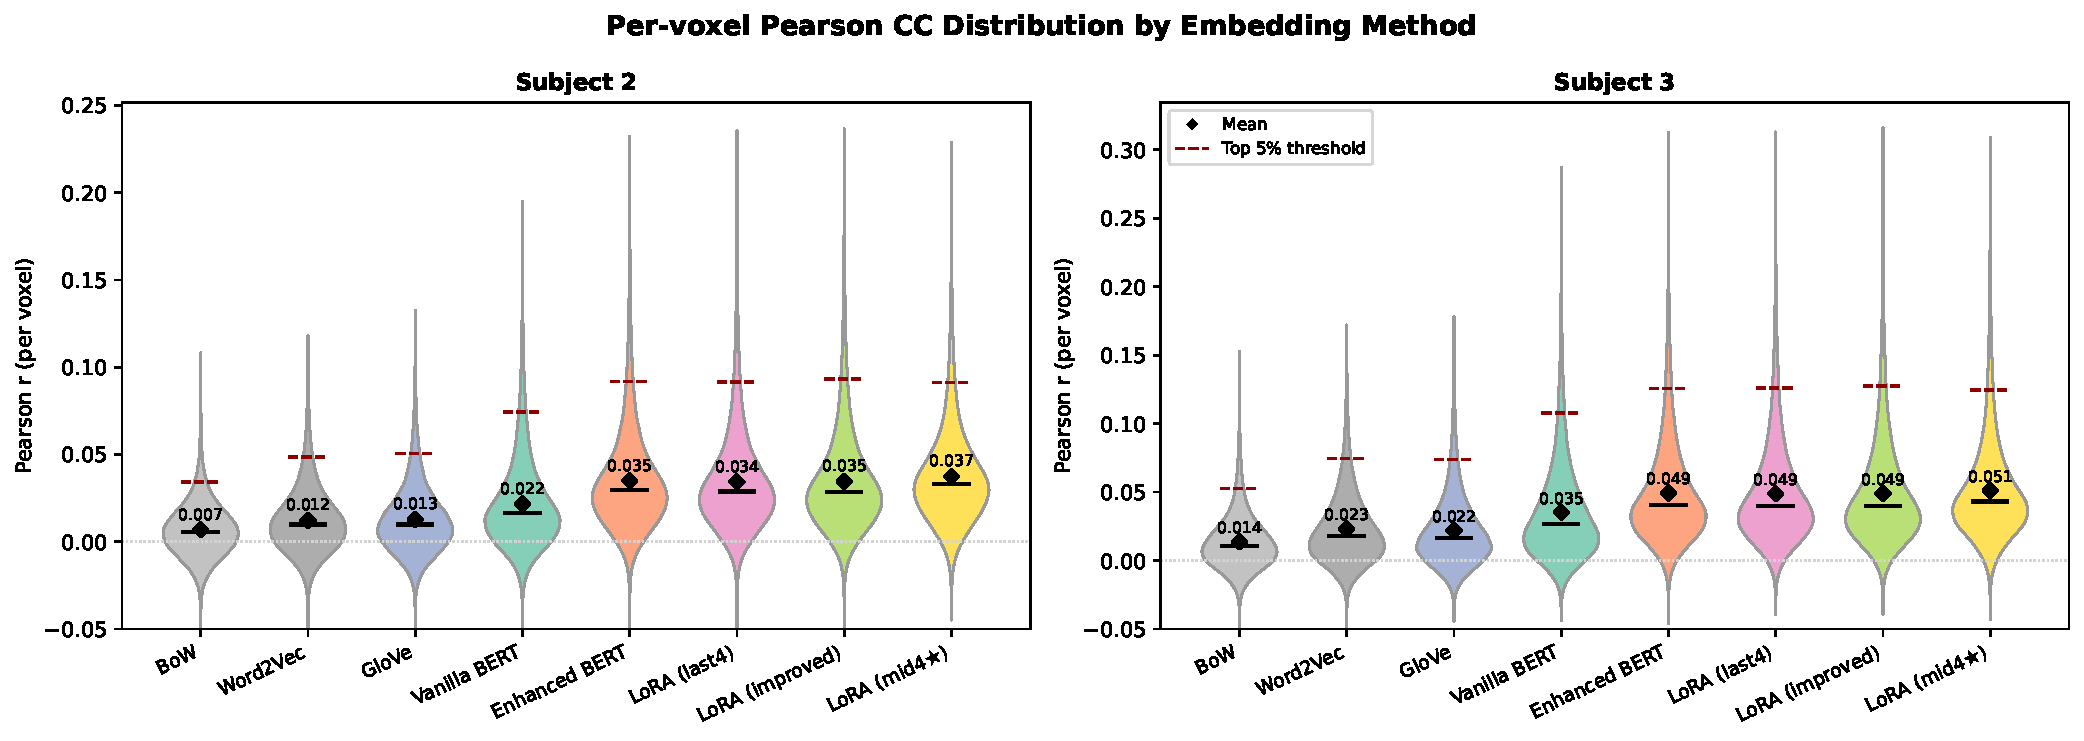
\includegraphics[width=\linewidth]{results/regression/fig1_cc_distributions.pdf}
  \caption{Per-voxel Pearson $r$ distribution for each embedding method,
           shown as violin plots.  Black diamonds ($\blacklozenge$) mark the
           mean; dashed red lines mark the 95th-percentile threshold.
           Left: Subject~2 (94{,}251 voxels).  Right: Subject~3 (95{,}556
           voxels).  Methods are ordered from left to right in increasing
           mean performance.}
  \label{fig:cc_dist}
\end{figure}


\subsection{Statistical Significance of Method Gains}


Figure~\ref{fig:method_prog} summarises the progression quantitatively,
showing the percent gain in mean $r$ over the GloVe baseline for each method
and both subjects.

Every consecutive step in the eight-method hierarchy produces a statistically
significant improvement ($p < 10^{-15}$, paired Wilcoxon signed-rank test on
all ${\sim}94{,}000$ per-voxel differences), with one exception: the transition
from Enhanced BERT to LoRA (last4) is not significant in s2 ($p \approx 1.0$),
consistent with the $<2\%$ numerical gap between those methods.  The
non-contextual tier transitions---BoW$\to$Word2Vec and Word2Vec$\to$GloVe---are
also highly significant, reflecting genuine semantic gains at each step even
among static embeddings.  The gain from LoRA (last4) to LoRA (mid4) is strongly
significant ($p < 10^{-15}$), confirming that the layer-selection
choice---middle layers 5--8 vs.\ final layers 9--12---has a genuine and
reproducible effect on cortical prediction.

Relative to GloVe, LoRA (mid4) achieves $+193\%$ mean-$r$ improvement on s2
and $+133\%$ on s3, while BoW falls $-46\%$/$-37\%$ below GloVe.
The diminishing returns from LoRA (improved) to LoRA (mid4) ($+$8.4\% on s2)
suggest that the architectural change in layer selection dominates over any
refinement in the fine-tuning recipe.

\begin{figure}[H]
  \centering
  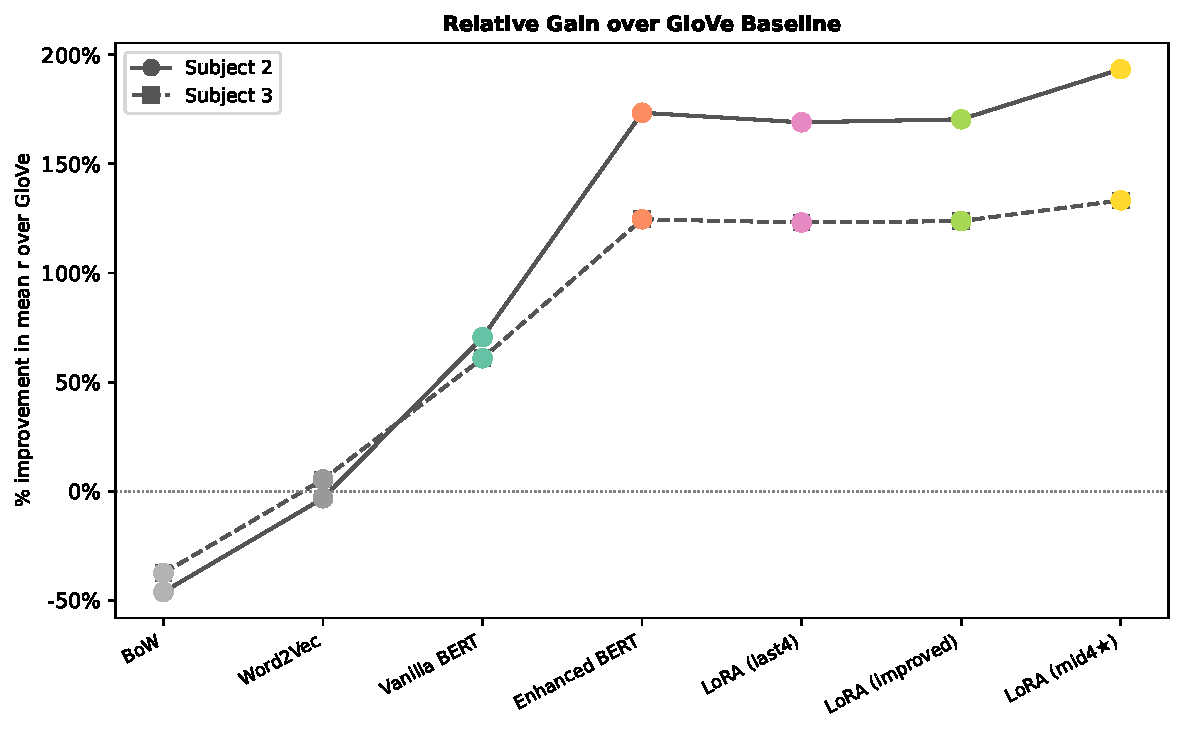
\includegraphics[width=0.8\linewidth]{results/regression/fig2_method_progression.pdf}
  \caption{Percent improvement in mean Pearson $r$ relative to the GloVe
           baseline for each non-GloVe method.  Circles and solid line:
           Subject~2; squares and dashed line: Subject~3.  Coloured dots
           follow the per-method colour scheme used throughout.  Negative
           values (BoW, Word2Vec on s2) indicate that those methods fall
           \emph{below} GloVe; BERT-based methods show large positive gains
           peaking at $+193\%$/$+133\%$ for LoRA (mid4).}
  \label{fig:method_prog}
\end{figure}


\subsection{Inter-Method Voxel-Ranking Correlation}

A natural question is whether different embedding families identify the
\emph{same} language-responsive voxels.  We measure this with the Spearman
rank correlation $\rho$ between per-voxel CC vectors for each pair of methods
within a subject (Figure~\ref{fig:intermethod}).

Four tiers of agreement emerge.
\textbf{(1) Within the non-contextual tier:}
BoW vs.\ Word2Vec ($\rho = 0.51$/$0.64$ on s2/s3) and BoW vs.\ GloVe
($\rho = 0.55$/$0.66$) show only moderate agreement, reflecting that one-hot
counts share some voxel-ranking signal with semantic vectors but miss the bulk
of it.  Word2Vec vs.\ GloVe is substantially higher ($\rho = 0.75$/$0.82$),
consistent with both methods producing semantically comparable 300-d dense
vectors trained on similar large-scale corpora.
\textbf{(2) Non-contextual vs.\ BERT:}
GloVe vs.\ any BERT variant spans $\rho = 0.56$--$0.63$ (s2) and
$0.69$--$0.75$ (s3), indicating that static distributional statistics share a
moderate portion of the brain-predictive signal with contextual representations
but capture a meaningfully different set of language-responsive voxels.
\textbf{(3) Vanilla BERT vs.\ fine-tuned BERT:}
$\rho \approx 0.80$--$0.81$ (s2) and $0.88$ (s3), reflecting the shared
pretrained backbone.  Notably, Enhanced BERT and LoRA (last4) are nearly
indistinguishable in which voxels they predict ($\rho = 0.957$/$0.973$),
confirming that podcast fine-tuning does not meaningfully shift the spatial
prediction pattern when reading from the upper layers.
\textbf{(4) Within the LoRA family:}
LoRA (last4) vs.\ LoRA (improved) yields $\rho = 0.977$/$0.984$, near-perfect
agreement confirming that the refined masking-and-window training recipe makes
negligible difference to which voxels benefit.  LoRA (last4) vs.\ LoRA (mid4),
however, drops to $\rho = 0.866$/$0.909$, a meaningful reduction showing that
changing the extraction layer from 9--12 to 5--8 genuinely redistributes
predictive power to a different set of brain regions---consistent with the
hypothesis that middle BERT layers are more broadly aligned with cortical
language processing than the task-specialised upper layers.

\begin{figure}[htbp]
  \centering
  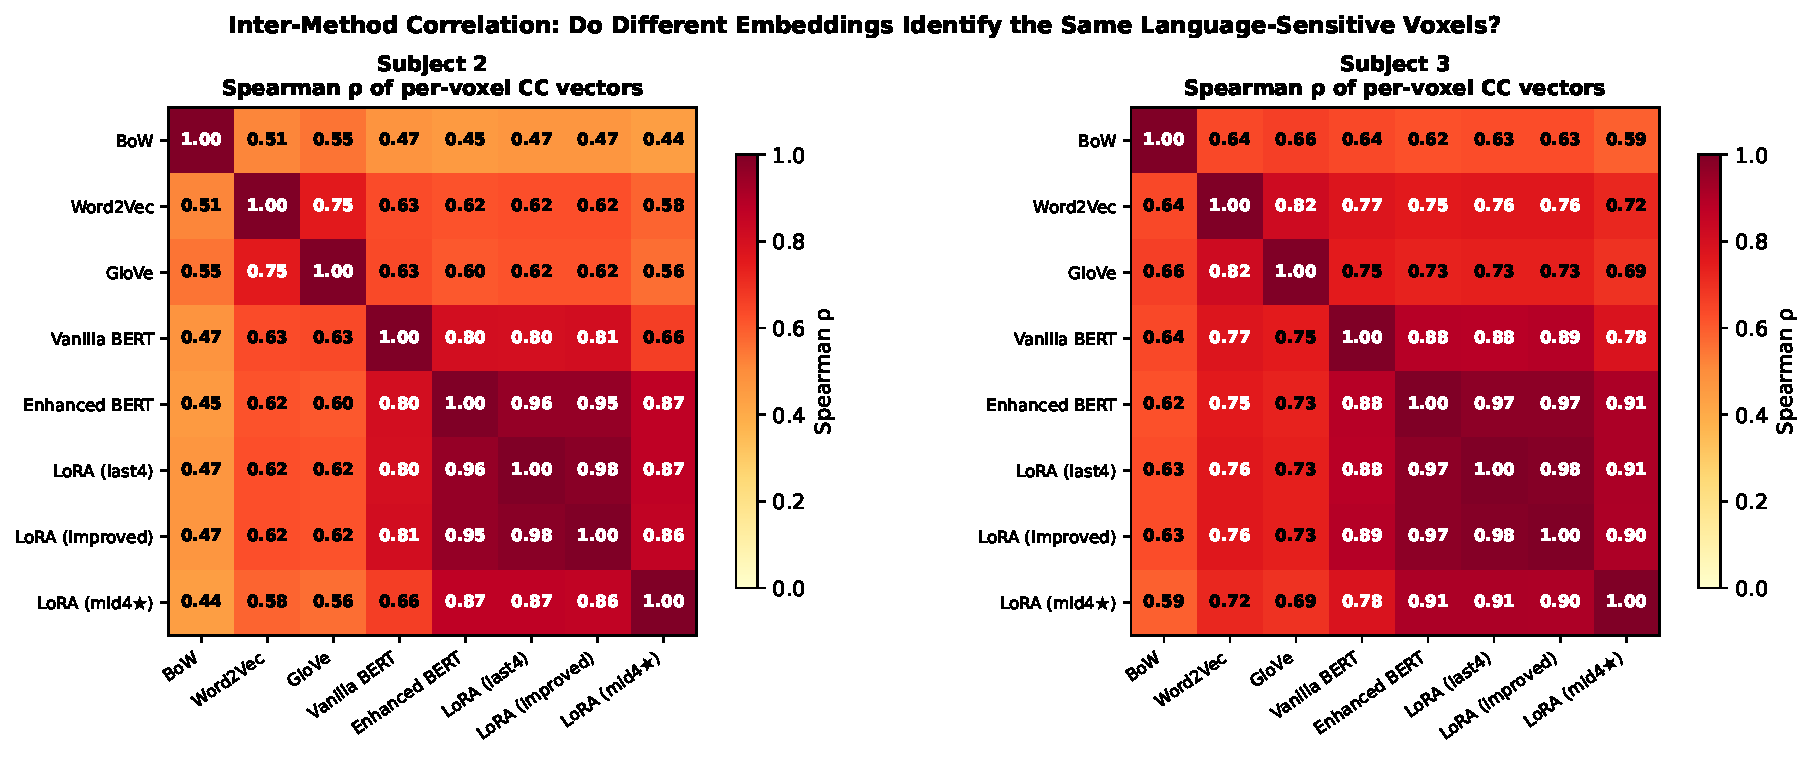
\includegraphics[width=\linewidth]{results/regression/fig3_intermethod_corr.pdf}
  \caption{Spearman rank correlation $\rho$ between per-voxel CC vectors for
           every method pair, computed within each subject.  Higher values mean
           the two methods rank voxels similarly in terms of language
           responsiveness.  Left: Subject~2.  Right: Subject~3.}
  \label{fig:intermethod}
\end{figure}



\graphicspath{{results/interpretation/}}
\documentclass[letterpaper,11pt]{article}

\usepackage[margin=1in]{geometry}
\setlength\parindent{0pt}
\setlength{\parskip}{0.7em}

\usepackage{titlesec}
\titlespacing*{\section}{0pt}{0.6\baselineskip}{0.2\baselineskip}
\titlespacing*{\subsection}{0pt}{0.4\baselineskip}{0.1\baselineskip}
\titlespacing*{\subsubsection}{0pt}{0.3\baselineskip}{0.1\baselineskip}

\usepackage{enumitem}
\setlist{nosep, topsep=2pt}

\usepackage{graphicx}
\graphicspath{{../results/interpretation/}}

\usepackage{subcaption}
\usepackage{booktabs}
\usepackage{amsmath}
\usepackage{amssymb}
\usepackage{bm}
\usepackage[hidelinks]{hyperref}

\title{Interpretation: SHAP and LIME Analysis --- Lab 3\\
       \large Connecting Language to fMRI, Stat 214, Spring 2026\vspace{-1em}}
\date{}

\begin{document}
\maketitle


\section{Interpretability Study}


Having established that the LoRA-fine-tuned BERT model with middle-layer pooling
(\texttt{finetuned\_lora\_mid4\_mean}) achieves the best voxelwise prediction
($\bar{r} = 0.0374$ for s2, $0.0512$ for s3), we ask \emph{what} each voxel is
responding to.  We apply two complementary attribution methods to the fitted
linear encoding model: closed-form linear SHAP identifies which BERT feature
dimensions drive predictions globally, and LIME isolates specific words within
individual stories that most influence particular voxels.  Both analyses are
conducted on the top-256 best-predicted voxels across two thematically distinct
test stories: \textit{On Approach to Pluto} (space exploration) and
\textit{Marry a Man Who Loves His Mother} (interpersonal relationships).
Predicted and observed BOLD response traces are shown for the four rank-1
voxels, with highlighted windows marking the local context used for LIME.


\subsection{Methods}


\subsubsection{SHAP for Linear Encoding Models}

The encoding model predicts voxel responses as $\hat{y}_i = \bm{X}_i \bm{w}$,
where $\bm{X}_i \in \mathbb{R}^{T \times 3072}$ is the delay-stacked embedding
matrix for story~$i$ and $\bm{w} \in \mathbb{R}^{3072}$ is the ridge-regression
weight vector for a given voxel.  Because $\bm{X}$ is z-scored before fitting,
the expected background value is zero and the linear SHAP attribution simplifies
to a closed form: the contribution of feature dimension~$j$ at time step~$t$ is
\begin{equation}
  \phi_j(x) = w_j (x_j - \mathbb{E}[x_j])
  \label{eq:shap}
\end{equation}
Global feature importance aggregates over the top-256 voxels:
\begin{equation}
  I_j = \sum_{v \in \mathcal{V}_{256}}
        \bigl|\phi_j^{(v)}\bigr|_{\text{mean}} \cdot \bigl|r_v\bigr|,
\end{equation}
where the outer weight $|r_v|$ up-weights voxels with stronger test correlations.
The 3072 feature dimensions correspond to four hemodynamic delay blocks
(delays 1--4\,TR $= 2$--8\,s), each of size 768 (the BERT hidden dimension).
We report importance both at the full feature level (3072 dims) and aggregated
across delay blocks to the 768 BERT dimension level.

Per-story word attribution maps each word to the TR in which it falls and
assigns the aggregate SHAP magnitude for that TR:
$\text{score}(w) = \sum_j |\phi_j(t_w)|$,
where $t_w$ is the TR index of word~$w$.  Because multiple words share the same
TR (at $\sim$3\,words/s with TR\,=\,2\,s, each TR contains up to six words),
words within the same TR receive identical scores.  This TR-resolution limitation
is addressed by LIME, which operates at the individual-word level.

\subsubsection{LIME with Word Masking}

LIME~(Ribeiro et al., 2016) approximates the local behavior of the encoding
model around a given input story by fitting a sparse linear surrogate on
perturbed inputs.  We represent each story as a binary vector over its unique
word types and generate 300 perturbations by randomly masking subsets of words.
Masking is implemented by zeroing all delay-block contributions of a word's
TR in the pre-built design matrix $\bm{X}$, preserving the original temporal
structure of surrounding context.  The ridge model then predicts the response
for each perturbed design matrix, and a weighted ridge regression on the binary
perturbation vectors fits the local linear surrogate.  The resulting
coefficients give each word a positive or negative contribution to the predicted
BOLD response of a target voxel.

The local window for LIME is defined as the 5-TR peak-response segment
(yellow shaded region in the response trace figures), identified as the
contiguous window with the highest mean absolute predicted BOLD signal during
that story.  Surrogate predictions average the model output across this
window, so LIME coefficients reflect how each word shifts the response
specifically during the most informative portion of the story.

We apply LIME to the three highest-ranked voxels (by test correlation $r$) for
each story, reporting the top positive contributors.


\subsection{SHAP Results}


\subsubsection{Dominant BERT Dimensions}

Figure~\ref{fig:shap_bertdim} shows the top-20 BERT dimensions by aggregate
SHAP importance for each subject.  The importance is broadly distributed across
all 768 dimensions with no single dominant axis, reflecting the high
dimensionality of the contextual embeddings.

\begin{figure}[H]
  \centering
  \begin{subfigure}[b]{0.48\textwidth}
    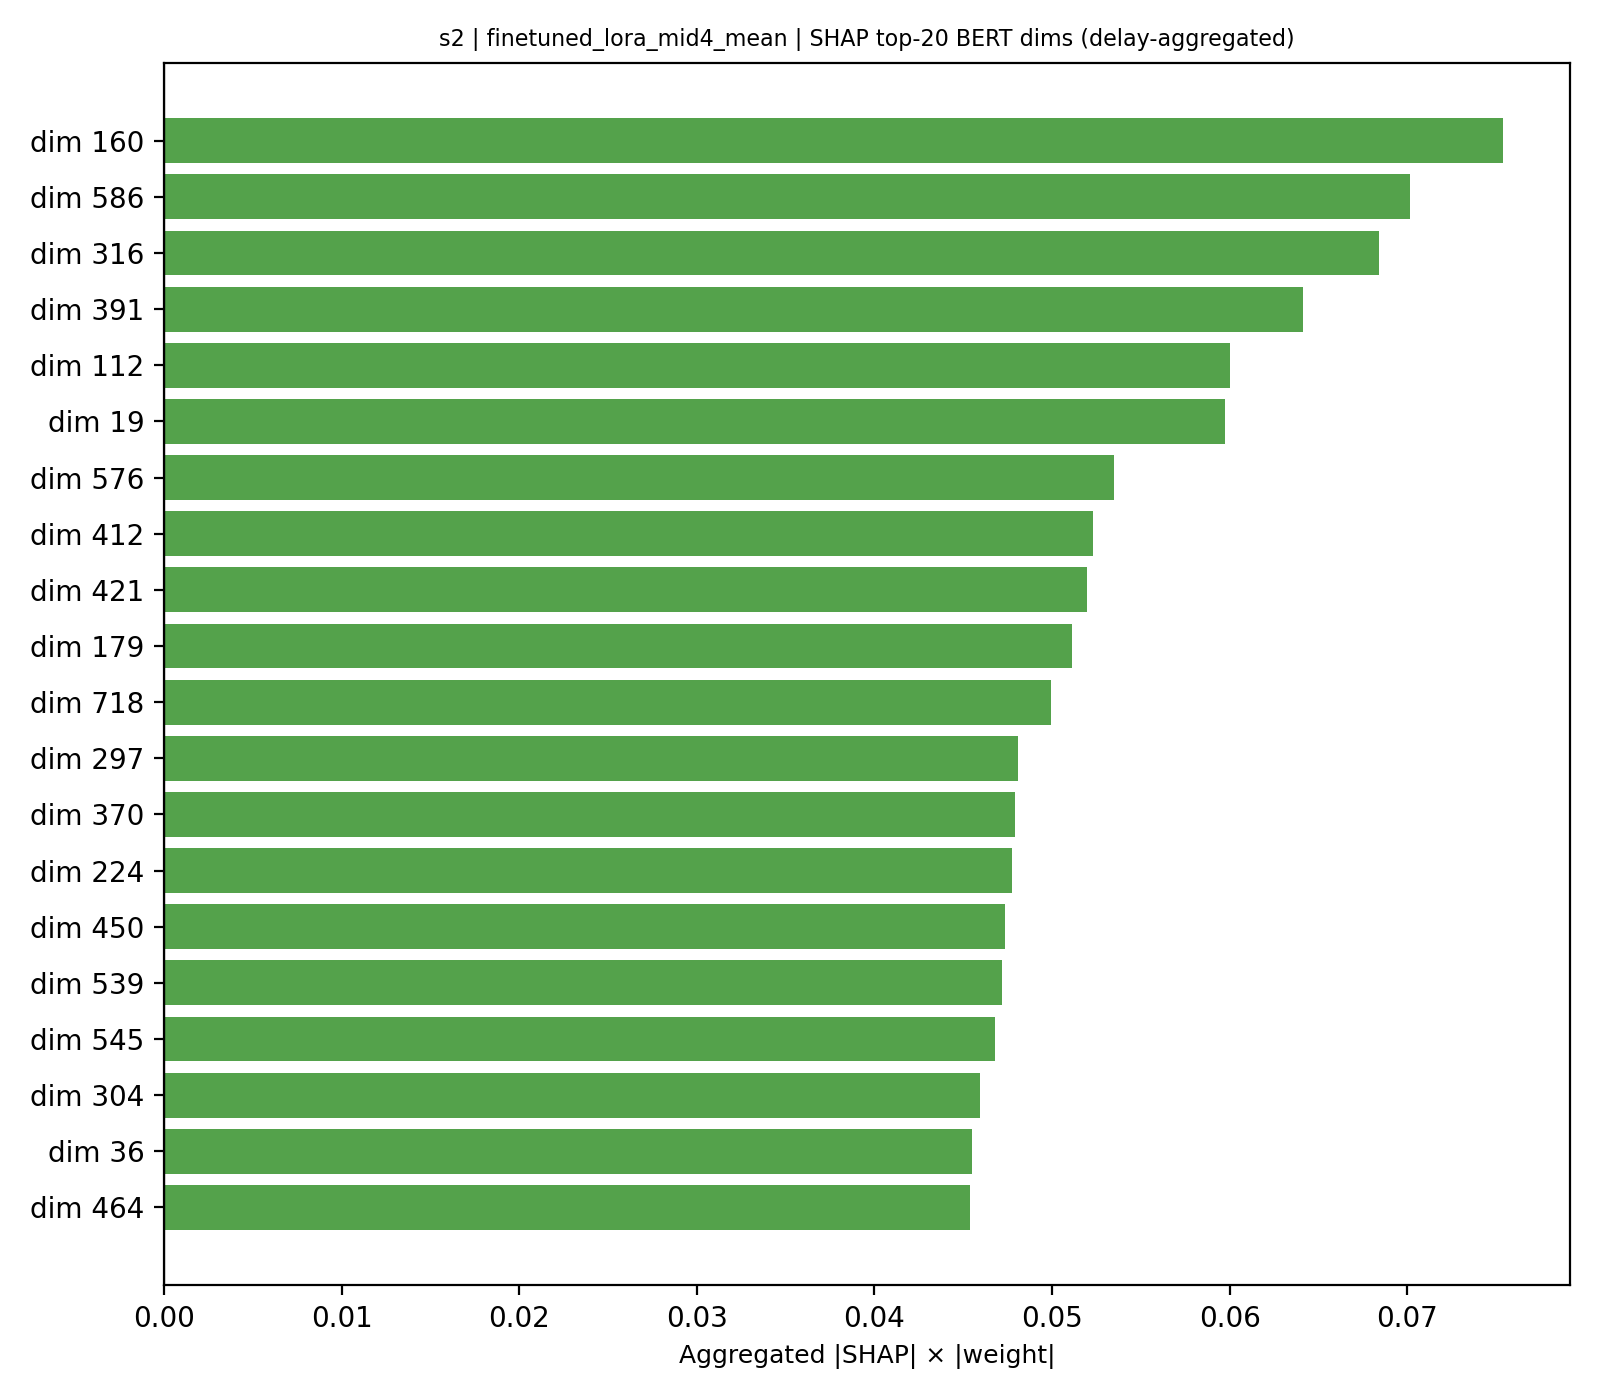
\includegraphics[width=\textwidth]{s2/finetuned_lora_mid4_mean/shap/s2_finetuned_lora_mid4_mean_shap_bert_dim_top20.png}
    \caption{Subject s2}
  \end{subfigure}
  \hfill
  \begin{subfigure}[b]{0.48\textwidth}
    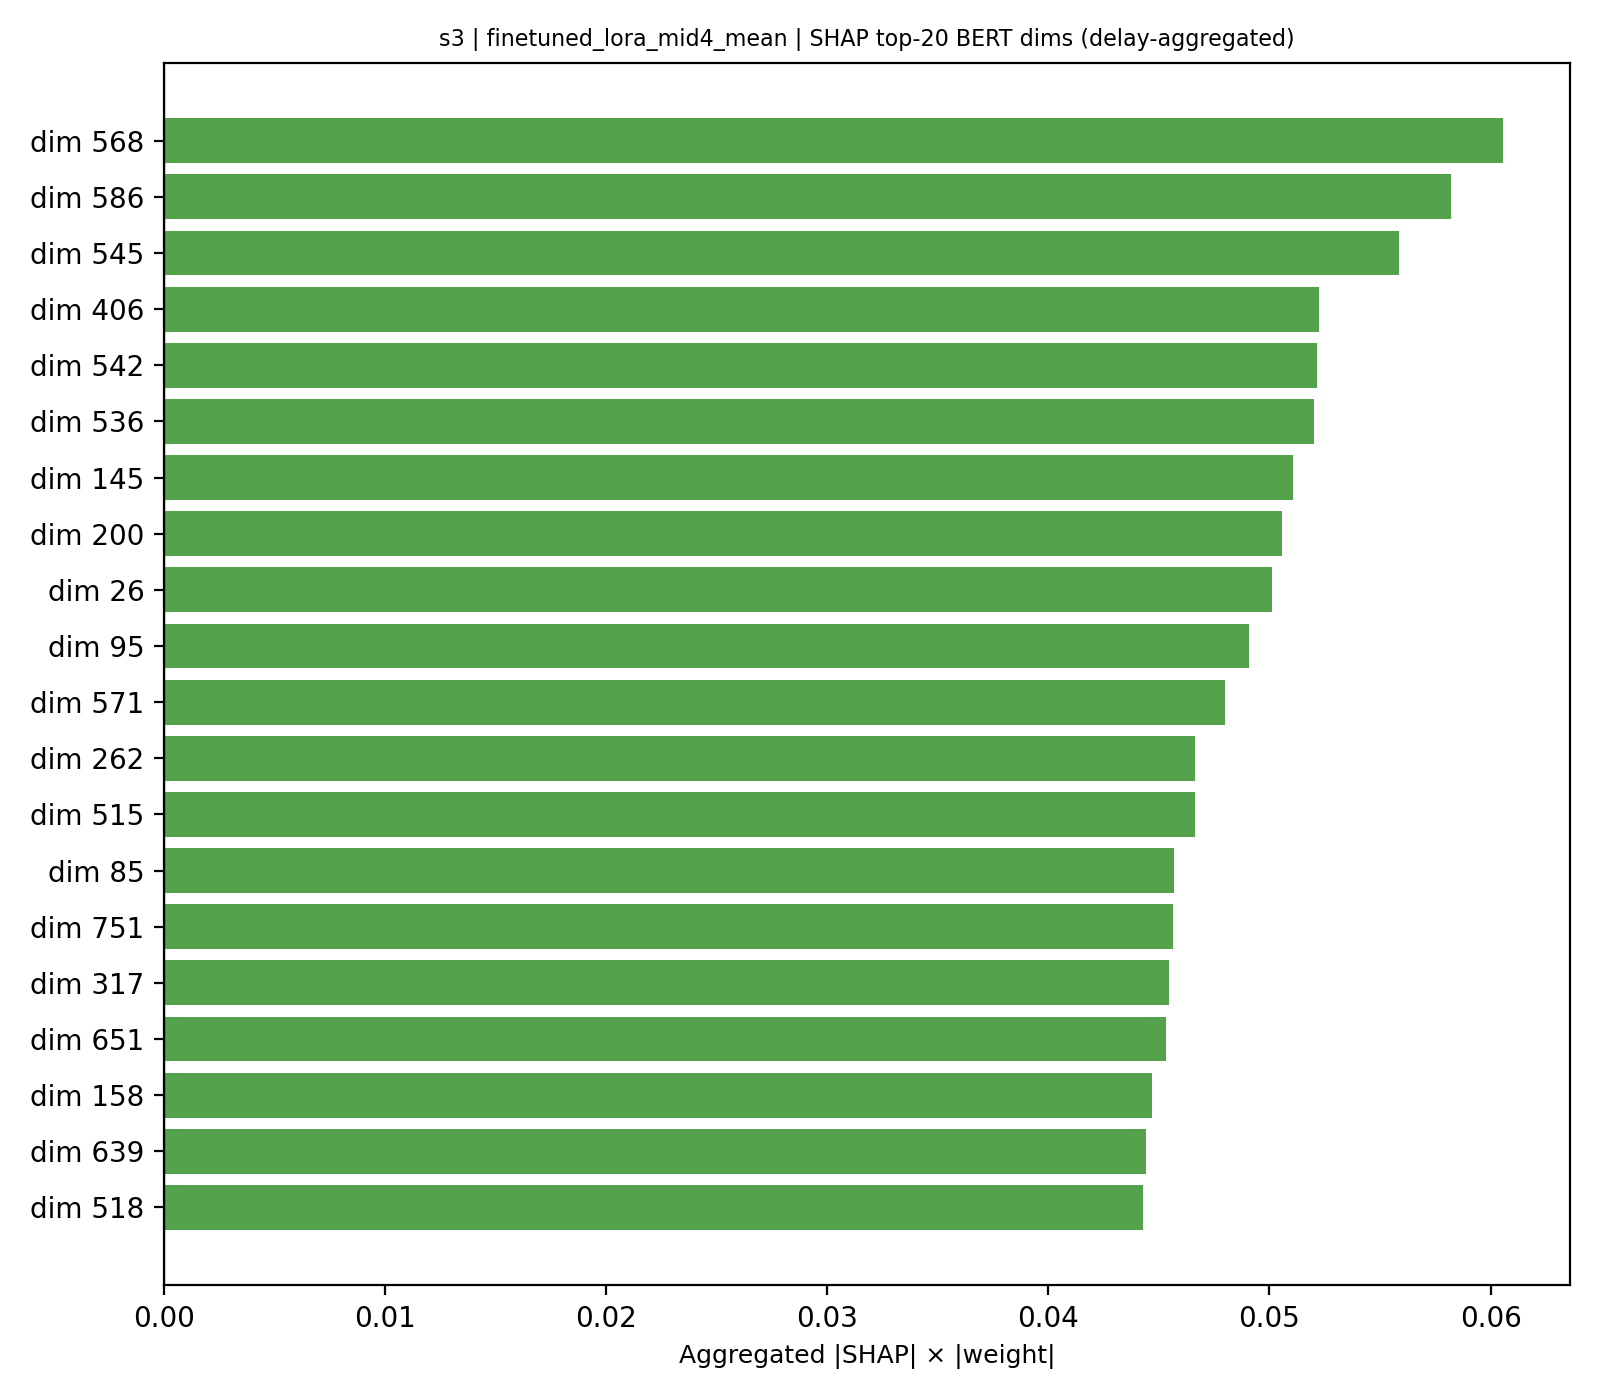
\includegraphics[width=\textwidth]{s3/finetuned_lora_mid4_mean/shap/s3_finetuned_lora_mid4_mean_shap_bert_dim_top20.png}
    \caption{Subject s3}
  \end{subfigure}
  \caption{Top-20 BERT dimensions by aggregated SHAP importance for the
           \texttt{finetuned\_lora\_mid4\_mean} model.  Each bar is the mean
           absolute SHAP value across the top-256 voxels, weighted by test
           correlation.  The importance is distributed across many dimensions,
           with no single axis dominating.}
  \label{fig:shap_bertdim}
\end{figure}

Despite the distributed pattern, several dimensions recur across subjects.
BERT dimension~586 ranks 2nd for both s2 and s3, and dimension~539 appears in
the top-10 for both (Table~\ref{tab:top_bertdims}).  The importance values for
s2 are consistently higher (0.050--0.075) than for s3 (0.049--0.061), consistent
with the overall higher predictability of s3 spreading encoding signal across a
broader set of dimensions.

\begin{table}[ht]
  \centering
  \small
  \begin{tabular}{lrrr}
    \toprule
    & \multicolumn{2}{c}{Rank} & \\
    \cmidrule(lr){2-3}
    BERT dim & s2 & s3 & Shared \\
    \midrule
    586 & 2 & 2 & \checkmark \\
    539 & 8 & 5 & \checkmark \\
    160 & 1 & -- & \\
    19  & 2 & -- & \\
    545 & -- & 1 & \\
    536 & -- & 2 & \\
    \bottomrule
  \end{tabular}
  \caption{Selected BERT dimensions from the top-10 SHAP ranking.  Dimensions
           shared across subjects (586, 539) represent candidate universally
           brain-relevant semantic axes.}
  \label{tab:top_bertdims}
\end{table}



Examining importance at the full 3072-dimensional feature level reveals a
consistent pattern: for both subjects, the highest-ranked features overwhelmingly
belong to delay block~1 (1\,TR\,=\,2\,s lag).  Of the top-10 features for s2,
eight are from delay block~1; for s3, nine of ten.  The same BERT dimension
(e.g., dim~160 for s2) contributes at delay block~1 (rank~1) and again at
delay block~2 (rank~4), but with lower importance at the longer lag.

This dominance of the 2\,s lag is somewhat surprising given that the canonical
hemodynamic response function (HRF) peaks at approximately 5--6\,s.  It likely
reflects two factors: (1) ridge regression fits all four delays simultaneously
and can assign weight to early onsets of the neural response, and (2) naturalistic
narrative language exhibits strong temporal autocorrelation, so nearby lags carry
overlapping semantic information that inflates the apparent weight of short delays.



Figure~\ref{fig:shap_words} shows the top-20 words by SHAP score for each of the
two target stories for subject s2.  Because SHAP attribution operates at TR
resolution, words that co-occur within the same 2\,s window receive identical
scores; tied bars therefore reflect a shared high-salience time window rather
than individual word salience.

For the Pluto story, the dominant TRs contain age and temporal markers
(``year'', ``old'', ``five'', ``three'') clustered around a passage describing
the multi-year journey, along with motion verbs (``move'').  For the relationship
story, the dominant TR contains a dense cluster of physical-scene nouns
(``wooden'', ``chair'', ``propped'', ``foot'', ``against''), reflecting a
vivid spatial description that drives a concentrated burst of cortical activity.

\begin{figure}[H]
  \centering
  \begin{subfigure}[b]{0.48\textwidth}
    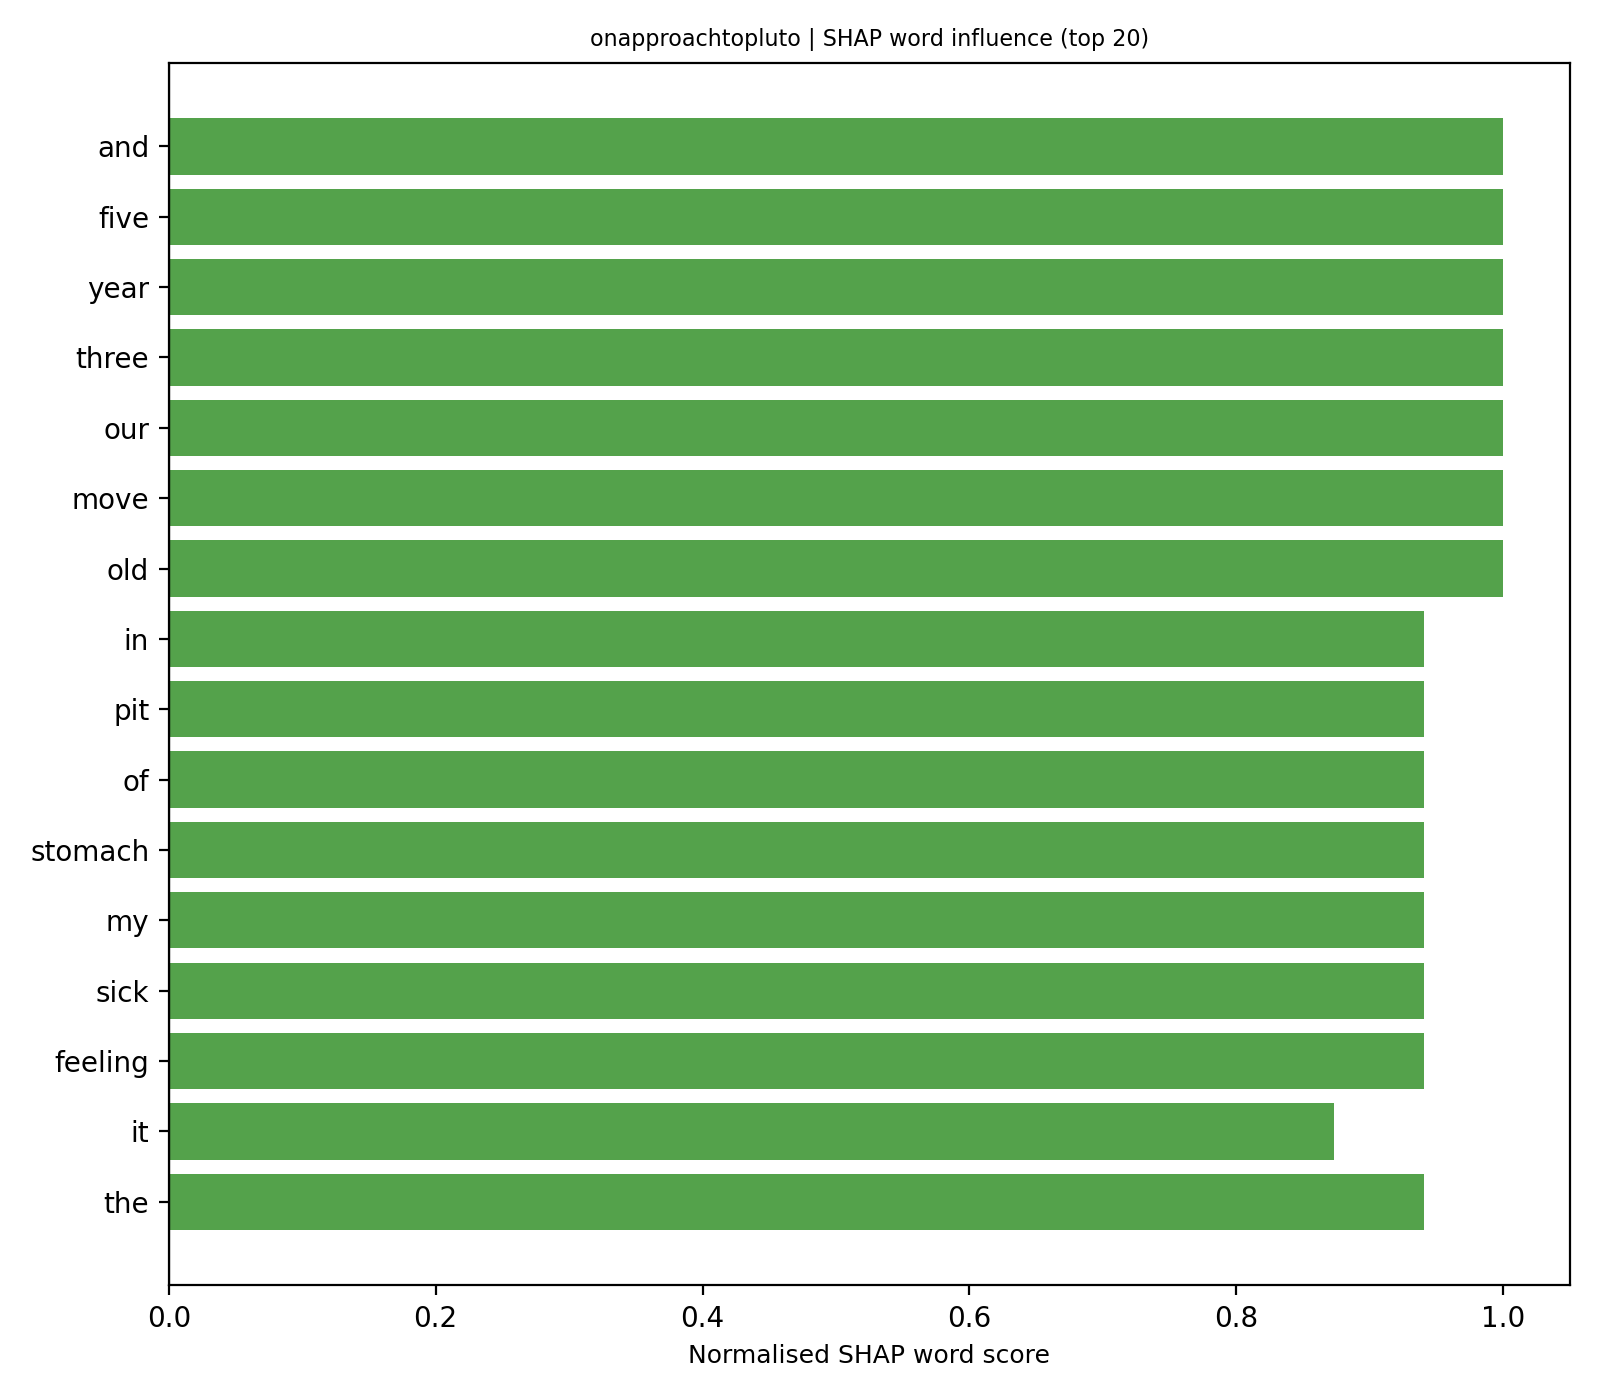
\includegraphics[width=\textwidth]{s2/finetuned_lora_mid4_mean/shap/s2_finetuned_lora_mid4_mean_onapproachtopluto_shap_words_top20.png}
    \caption{\textit{On Approach to Pluto}, s2}
  \end{subfigure}
  \hfill
  \begin{subfigure}[b]{0.48\textwidth}
    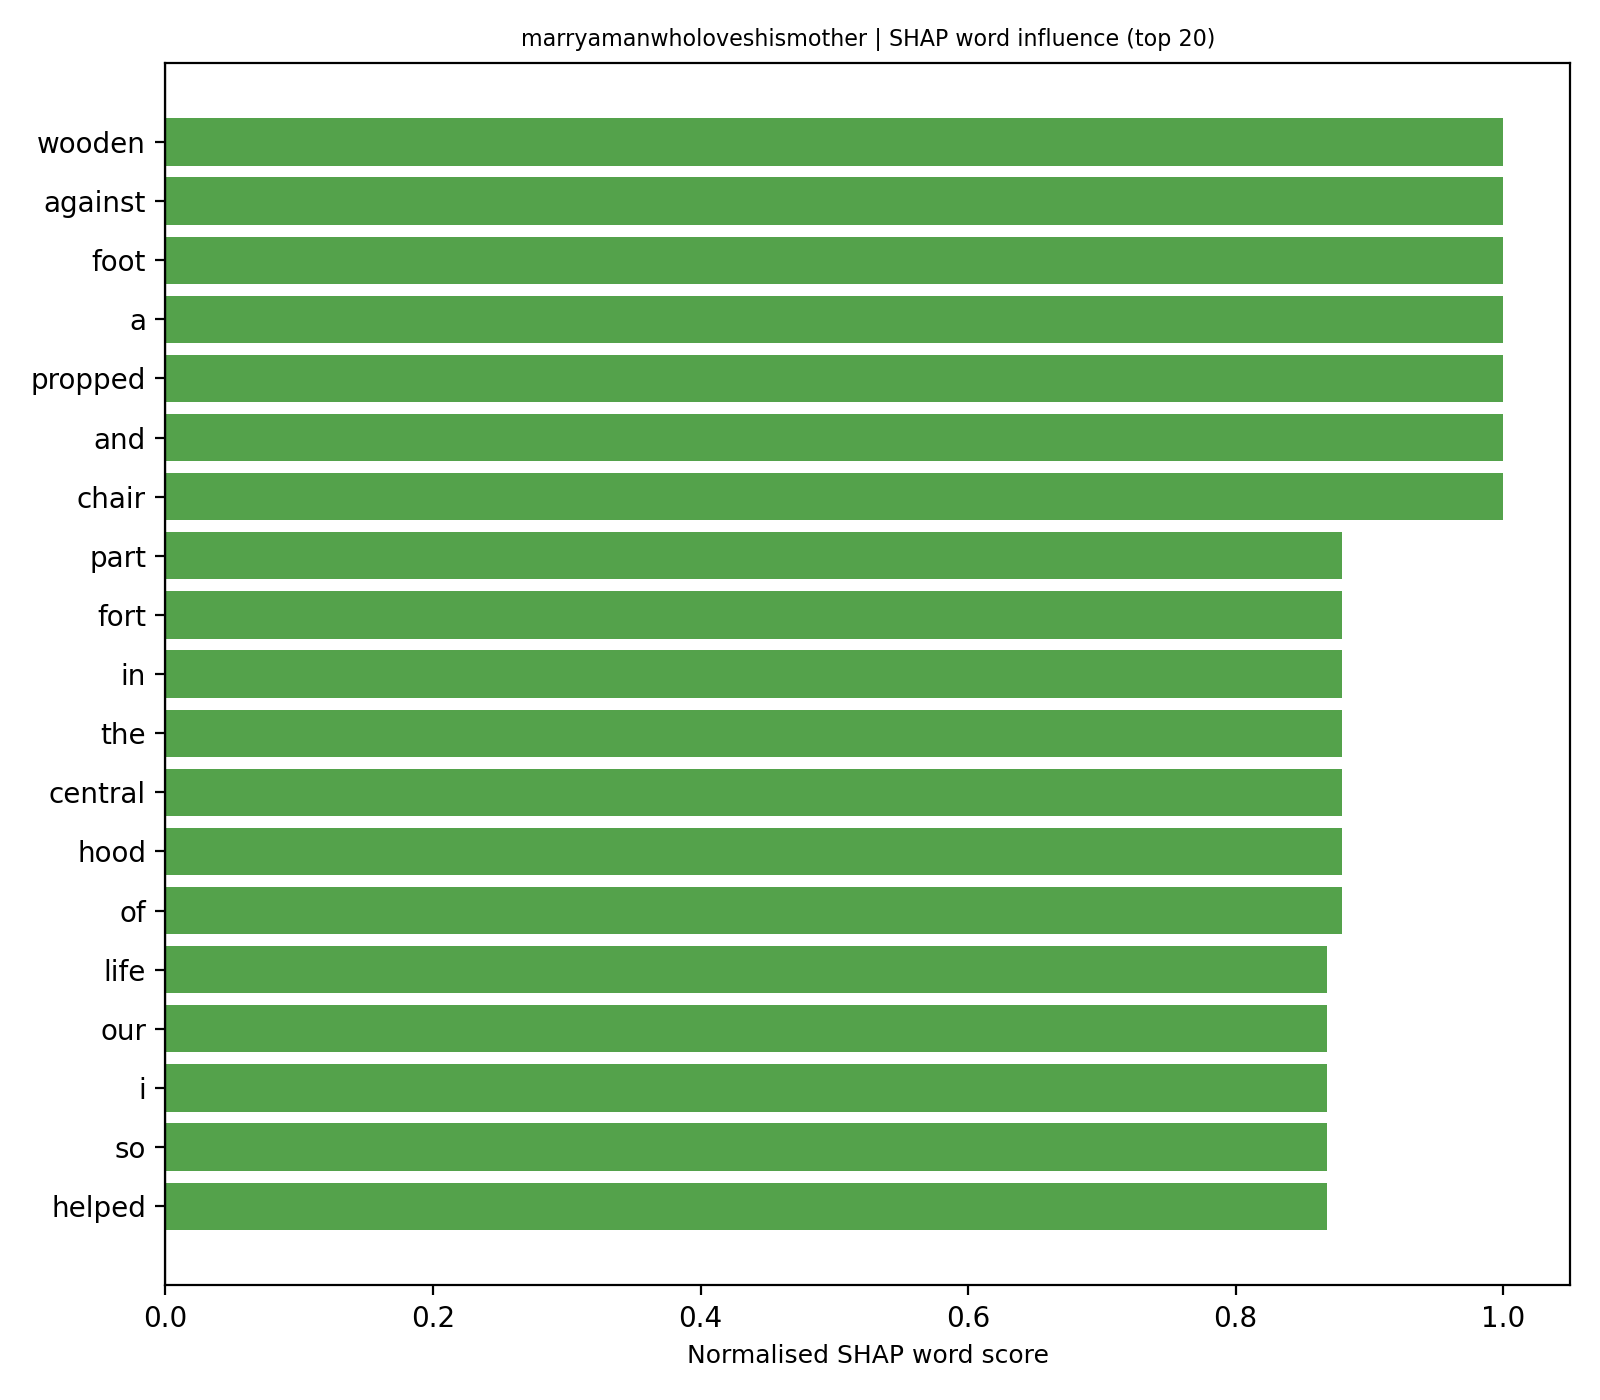
\includegraphics[width=\textwidth]{s2/finetuned_lora_mid4_mean/shap/s2_finetuned_lora_mid4_mean_marryamanwholoveshismother_shap_words_top20.png}
    \caption{\textit{Marry a Man\ldots}, s2}
  \end{subfigure}
  \caption{Top-20 words by SHAP score for subject s2.  Words sharing the same bar height belong to the same TR (2\,s window).  }
  \label{fig:shap_words}
\end{figure}


\subsection{LIME Results and Response Traces}


LIME resolves word-level attribution for the three top-ranked voxels per story.
Positive coefficients indicate words whose presence increases the voxel's
predicted BOLD response.  Response trace figures accompany the rank-1 voxels,
showing observed (blue) and predicted (orange) BOLD signals over the full story
with the yellow shaded region marking the 5-TR peak window used as the LIME
prediction target.

\subsubsection{Story: \textit{On Approach to Pluto} (Space Exploration)}

This story narrates the New Horizons spacecraft's multi-year journey to Pluto,
culminating in the July 2015 flyby.

\begin{figure}[H]
  \centering
  \begin{subfigure}[b]{0.48\textwidth}
    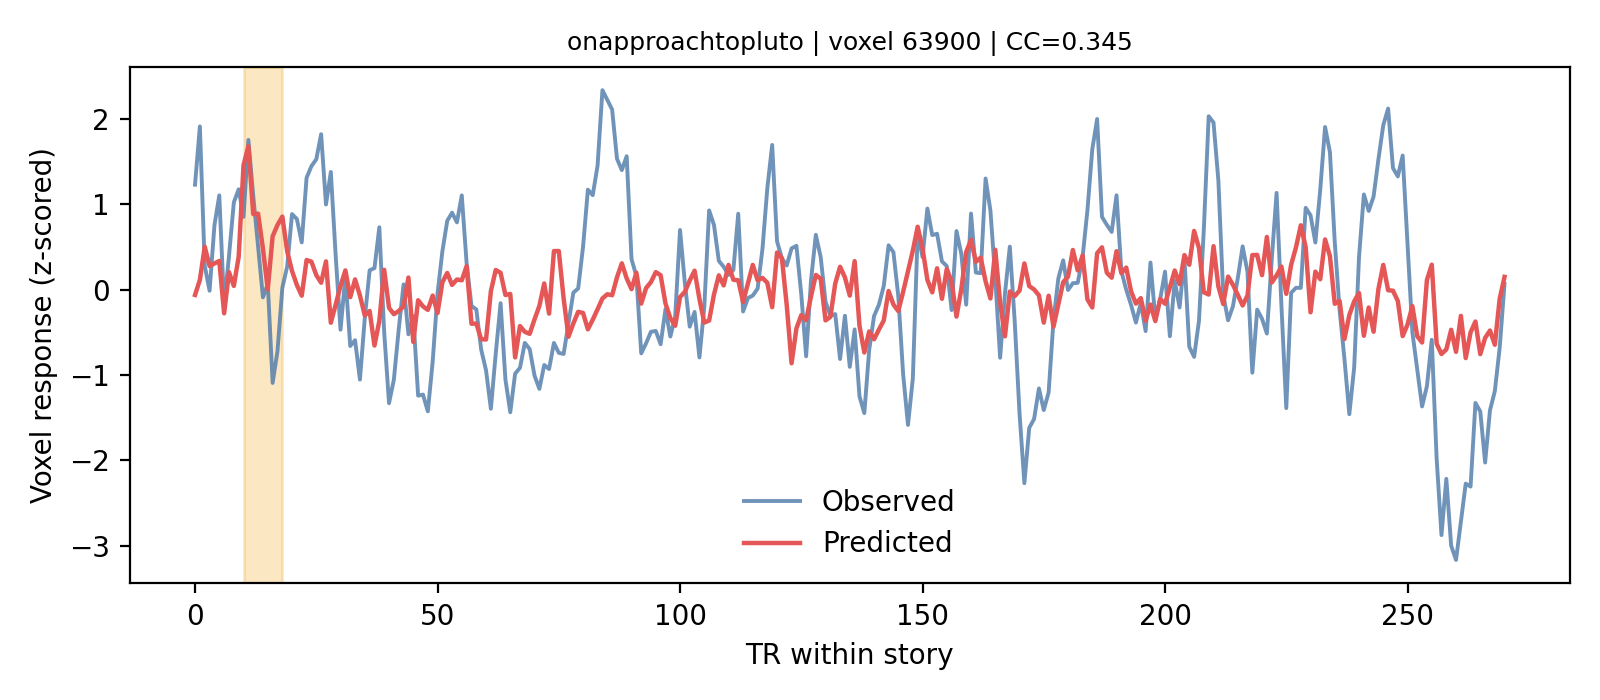
\includegraphics[width=\textwidth]{s2/finetuned_lora_mid4_mean/lime/onapproachtopluto/voxel63900_rank1_response.png}
    \caption{s2, rank-1 voxel (63900) --- response trace}
  \end{subfigure}
  \hfill
  \begin{subfigure}[b]{0.48\textwidth}
    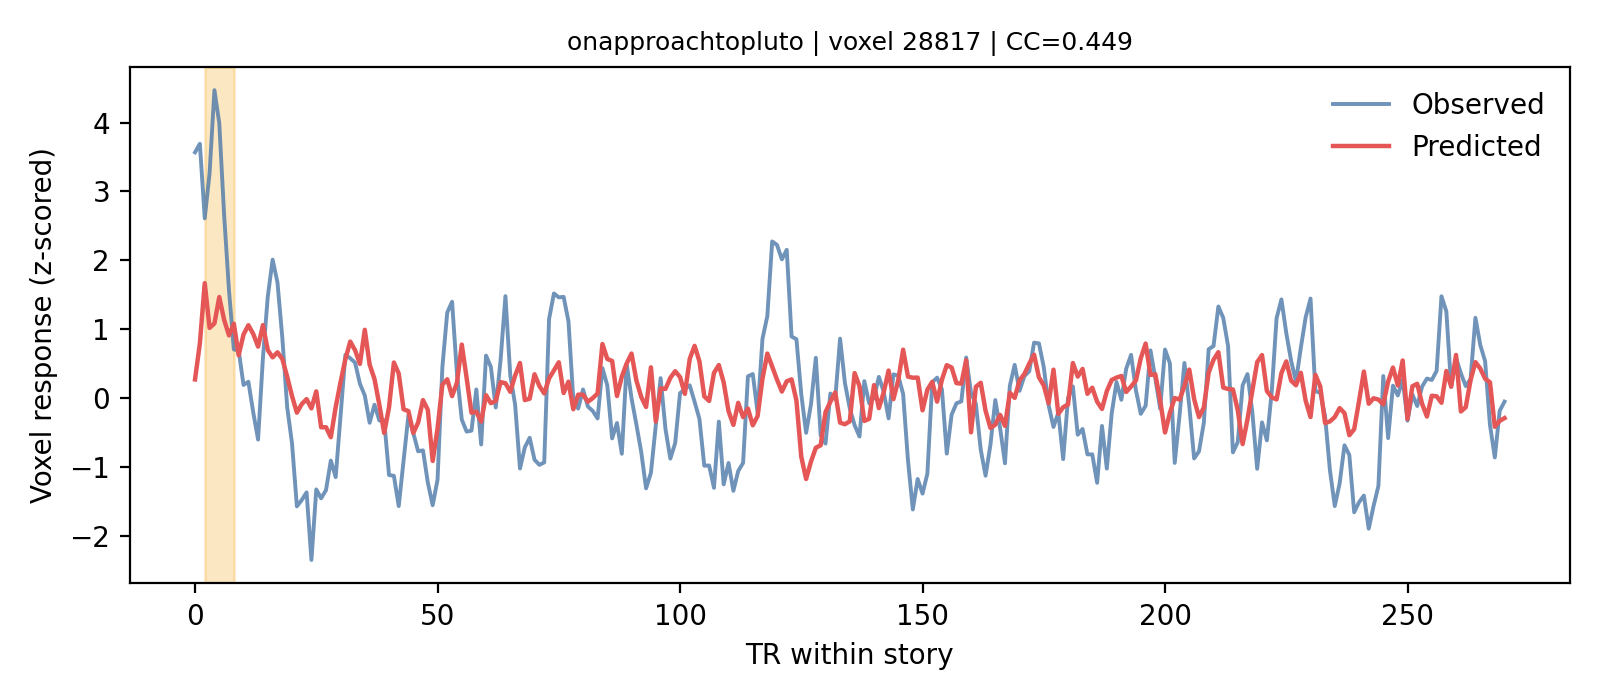
\includegraphics[width=\textwidth]{s3/finetuned_lora_mid4_mean/lime/onapproachtopluto/voxel28817_rank1_response.png}
    \caption{s3, rank-1 voxel (28817) --- response trace}
  \end{subfigure}
  \caption{Observed (blue) and predicted (orange) BOLD response for the
           rank-1 voxel per subject during \textit{On Approach to Pluto}.
           The yellow shaded region marks the 5-TR peak window where LIME
           attributions are computed.}
  \label{fig:resp_pluto}
\end{figure}

\begin{figure}[H]
  \centering
  \begin{subfigure}[b]{0.48\textwidth}
    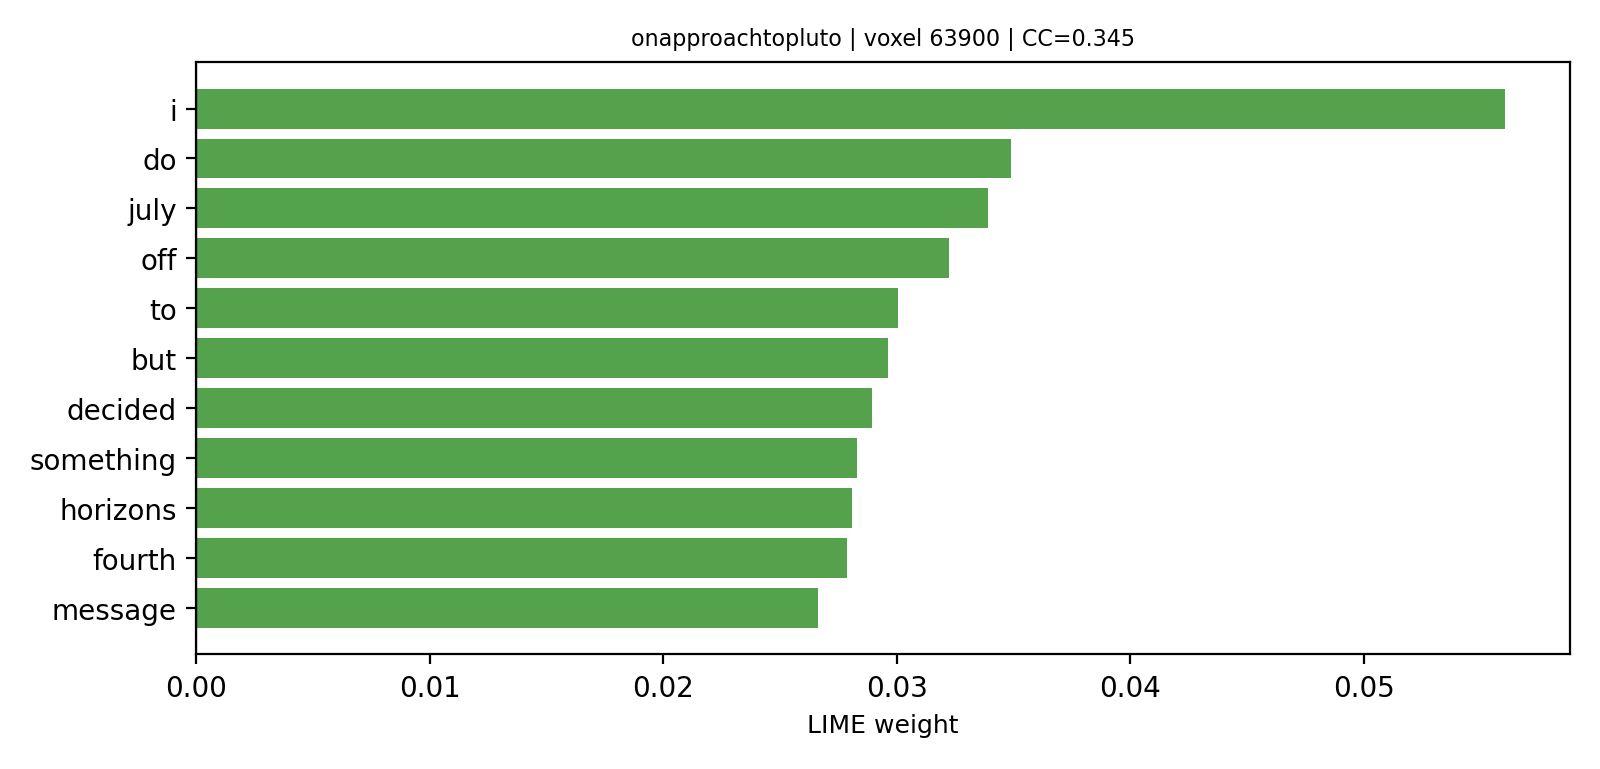
\includegraphics[width=\textwidth]{s2/finetuned_lora_mid4_mean/lime/onapproachtopluto/voxel63900_rank1_lime.png}
    \caption{s2, rank-1 voxel (63900)}
  \end{subfigure}
  \hfill
  \begin{subfigure}[b]{0.48\textwidth}
    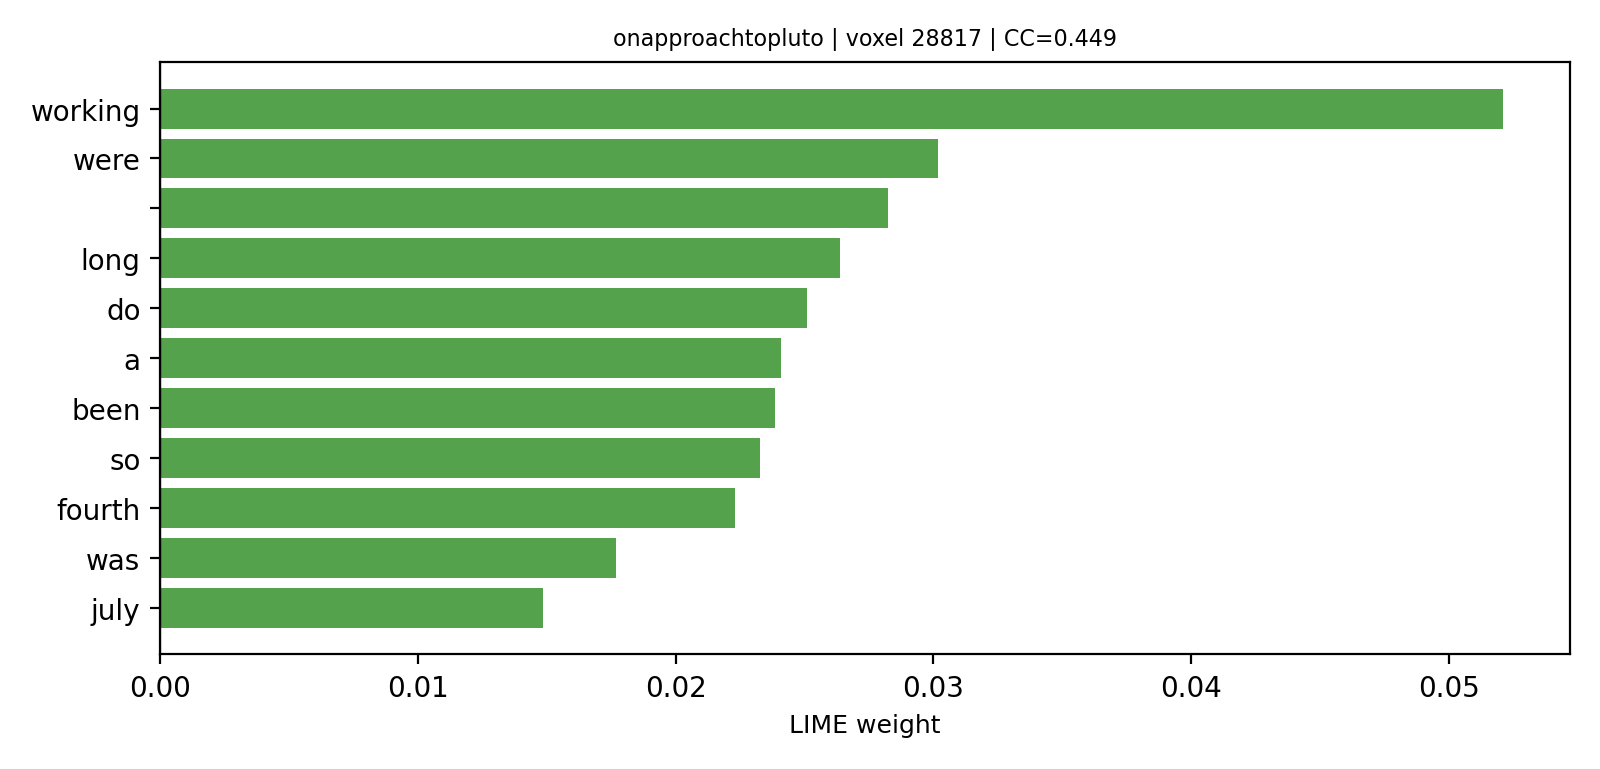
\includegraphics[width=\textwidth]{s3/finetuned_lora_mid4_mean/lime/onapproachtopluto/voxel28817_rank1_lime.png}
    \caption{s3, rank-1 voxel (28817)}
  \end{subfigure}
  \caption{LIME word importances for \textit{On Approach to Pluto}, rank-1 voxel
           per subject.  Attributions correspond to the highlighted window in
           Figure~\ref{fig:resp_pluto}.}
  \label{fig:lime_pluto_rank1}
\end{figure}



The response traces (Figure~\ref{fig:resp_pluto}) show that the model tracks the
broad temporal envelope of the BOLD signal, with the predicted trace following
the shape of the observed response.  The peak window falls in the mid-story
portion where the narration shifts from scene-setting to active mission
description.  Prediction quality is visibly higher during the highlighted peak
than at quiet story segments, consistent with the voxels being selectively driven
by dense semantic content rather than baseline speech.

Across both subjects and both top voxels, the leading LIME words are temporal
markers and goal-directed action verbs tied to the mission narrative:
\texttt{july}, \texttt{fourth}, \texttt{decided}, \texttt{horizons},
\texttt{working}, \texttt{long}.  The word \texttt{i} (the narrator's
first-person voice) is prominent for s2, likely reflecting moments of personal
reflection that co-occur with high-salience mission content.  The word
\texttt{fourth} appears in both subjects' rank-2 voxels alongside \texttt{july},
confirming that the same passage drives activity in spatially neighbouring
voxels.

\subsubsection{Story: \textit{Marry a Man Who Loves His Mother} (Interpersonal Relationships)}

This story depicts close interpersonal dynamics, domestic settings, and social
negotiations between characters.

\begin{figure}[H]
  \centering
  \begin{subfigure}[b]{0.48\textwidth}
    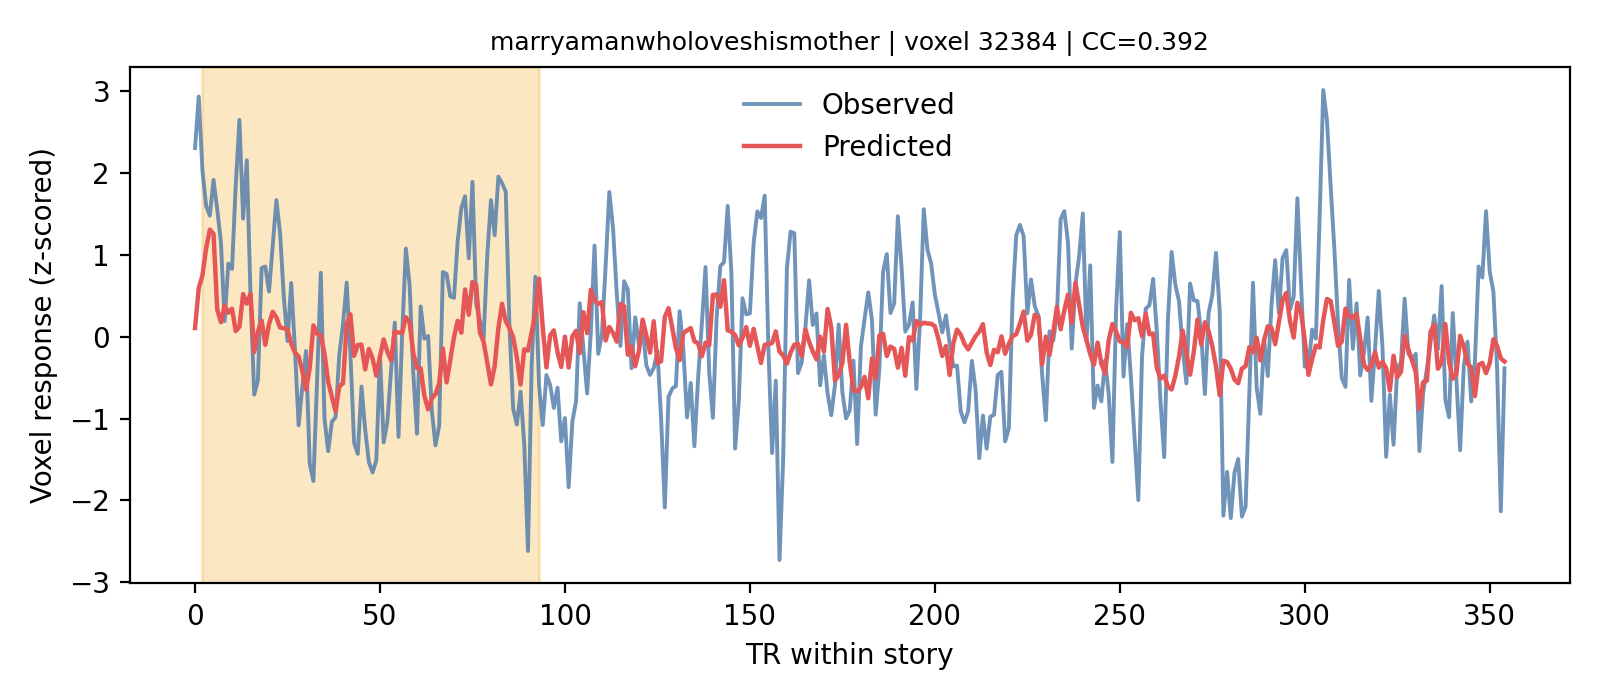
\includegraphics[width=\textwidth]{s2/finetuned_lora_mid4_mean/lime/marryamanwholoveshismother/voxel32384_rank1_response.png}
    \caption{s2, rank-1 voxel (32384) --- response trace}
  \end{subfigure}
  \hfill
  \begin{subfigure}[b]{0.48\textwidth}
    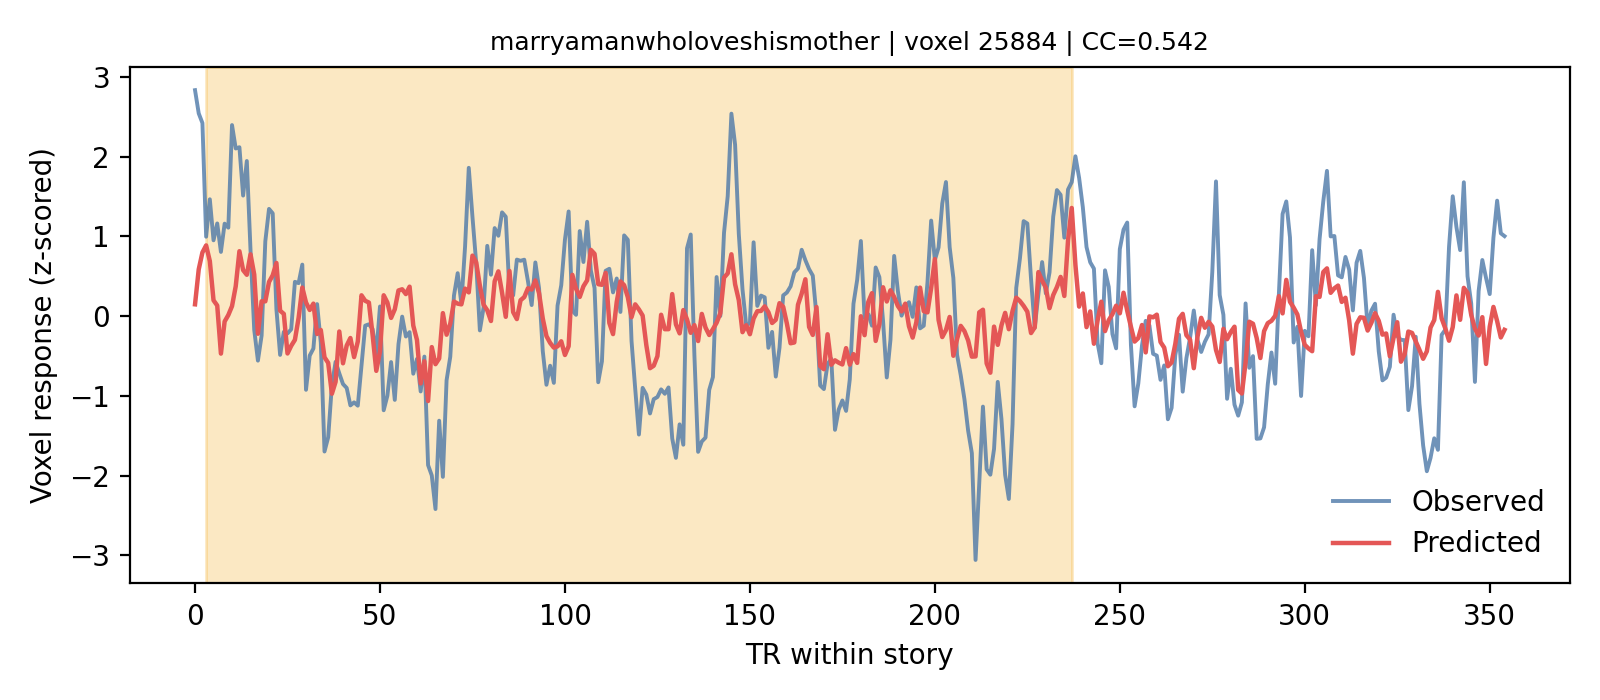
\includegraphics[width=\textwidth]{s3/finetuned_lora_mid4_mean/lime/marryamanwholoveshismother/voxel25884_rank1_response.png}
    \caption{s3, rank-1 voxel (25884) --- response trace}
  \end{subfigure}
  \caption{Observed and predicted BOLD response for the rank-1 voxel per subject
           during \textit{Marry a Man Who Loves His Mother}.  The yellow region
           marks the 5-TR peak window used by LIME.}
  \label{fig:resp_marry}
\end{figure}

\begin{figure}[H]
  \centering
  \begin{subfigure}[b]{0.48\textwidth}
    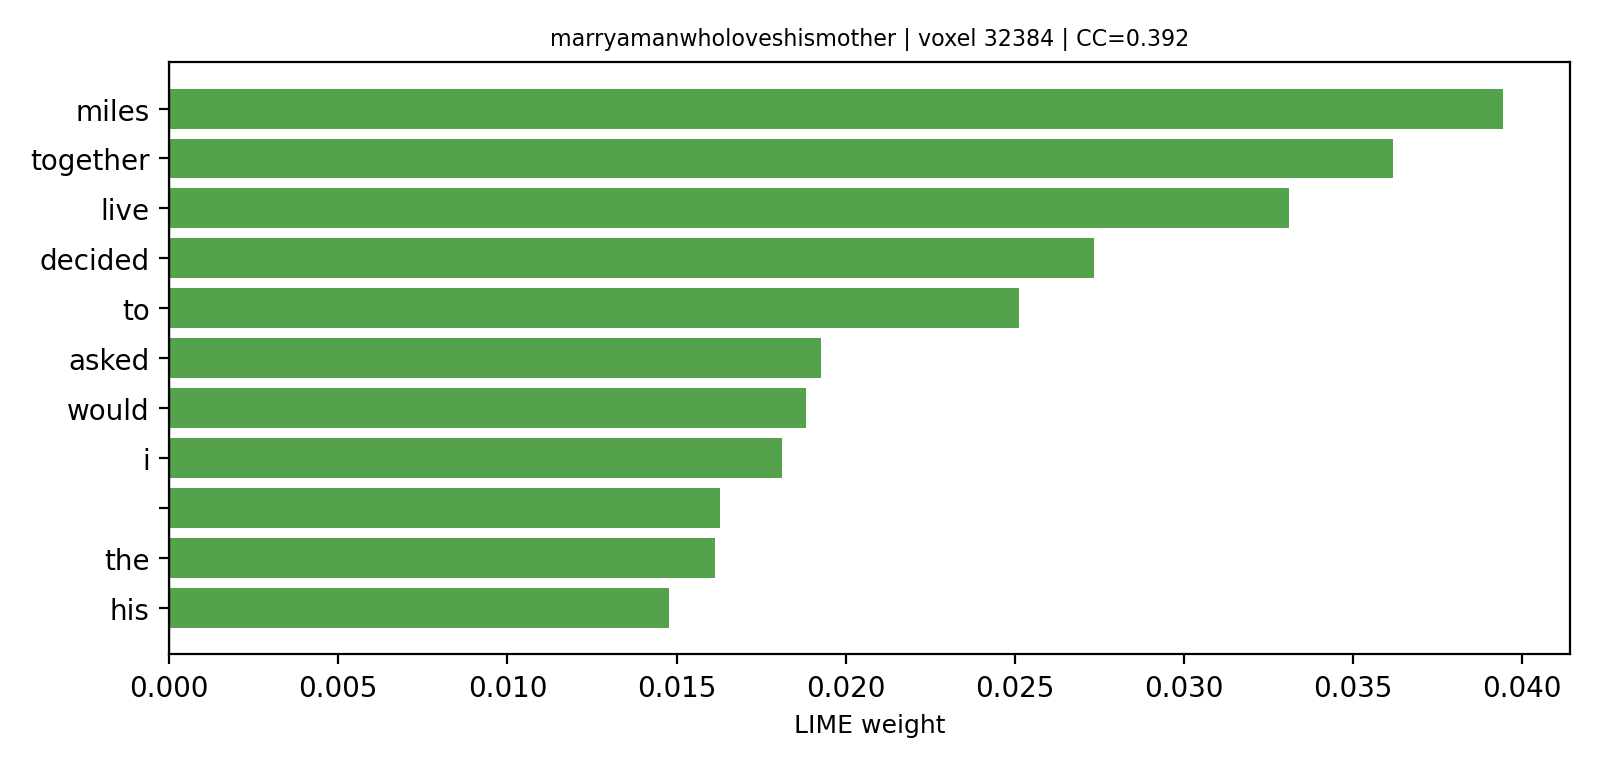
\includegraphics[width=\textwidth]{s2/finetuned_lora_mid4_mean/lime/marryamanwholoveshismother/voxel32384_rank1_lime.png}
    \caption{s2, rank-1 voxel (32384)}
  \end{subfigure}
  \hfill
  \begin{subfigure}[b]{0.48\textwidth}
    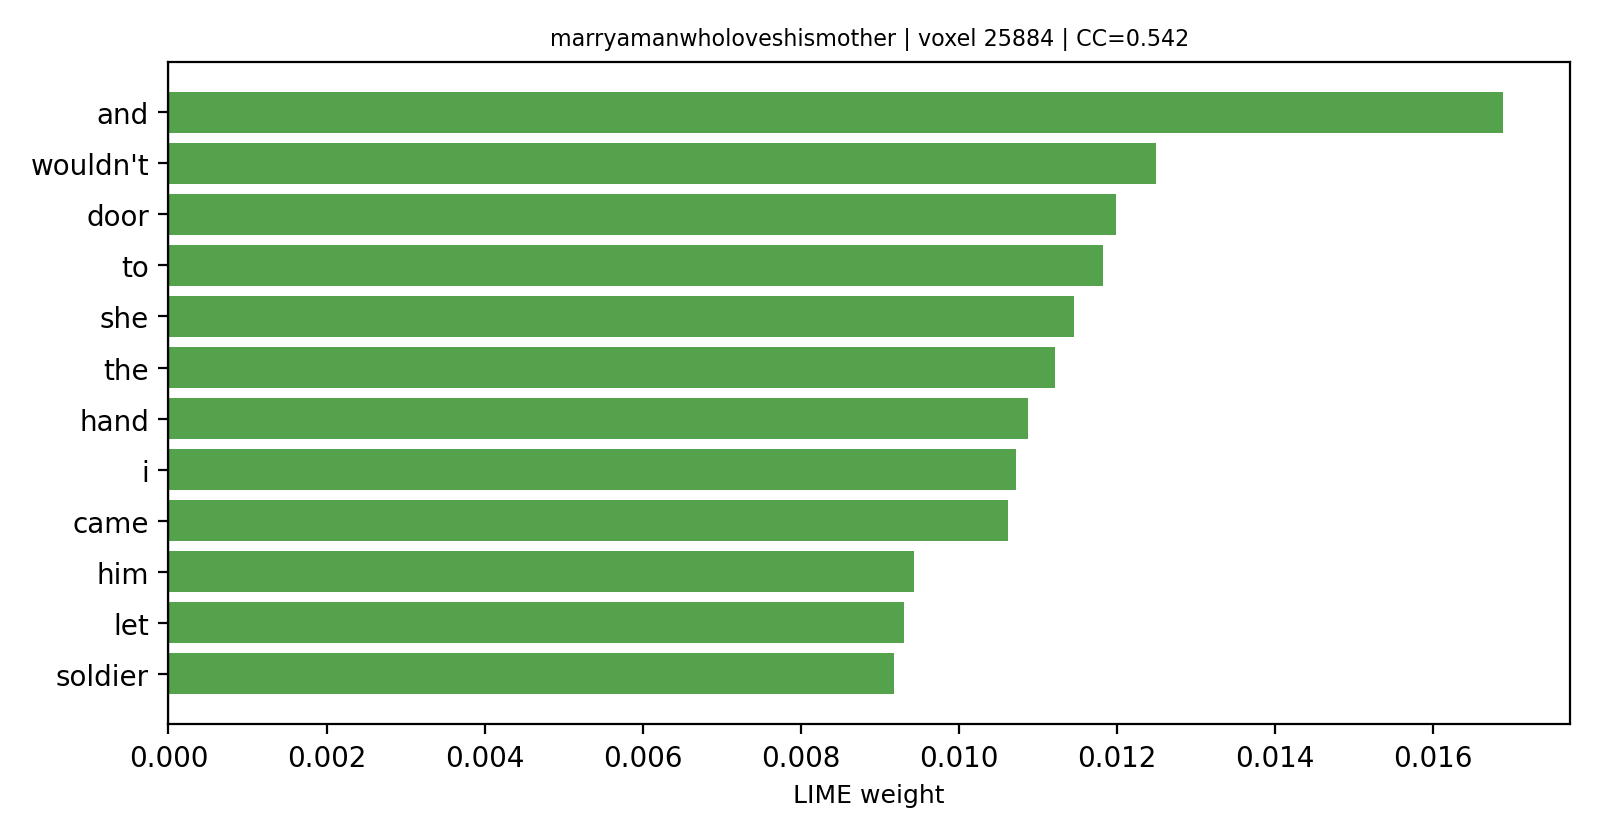
\includegraphics[width=\textwidth]{s3/finetuned_lora_mid4_mean/lime/marryamanwholoveshismother/voxel25884_rank1_lime.png}
    \caption{s3, rank-1 voxel (25884)}
  \end{subfigure}
  \caption{LIME word importances for \textit{Marry a Man Who Loves His Mother},
           rank-1 voxel per subject.  Attributions correspond to the highlighted
           window in Figure~\ref{fig:resp_marry}.}
  \label{fig:lime_marry_rank1}
\end{figure}

\begin{figure}[H]
  \centering
  \begin{subfigure}[b]{0.48\textwidth}
    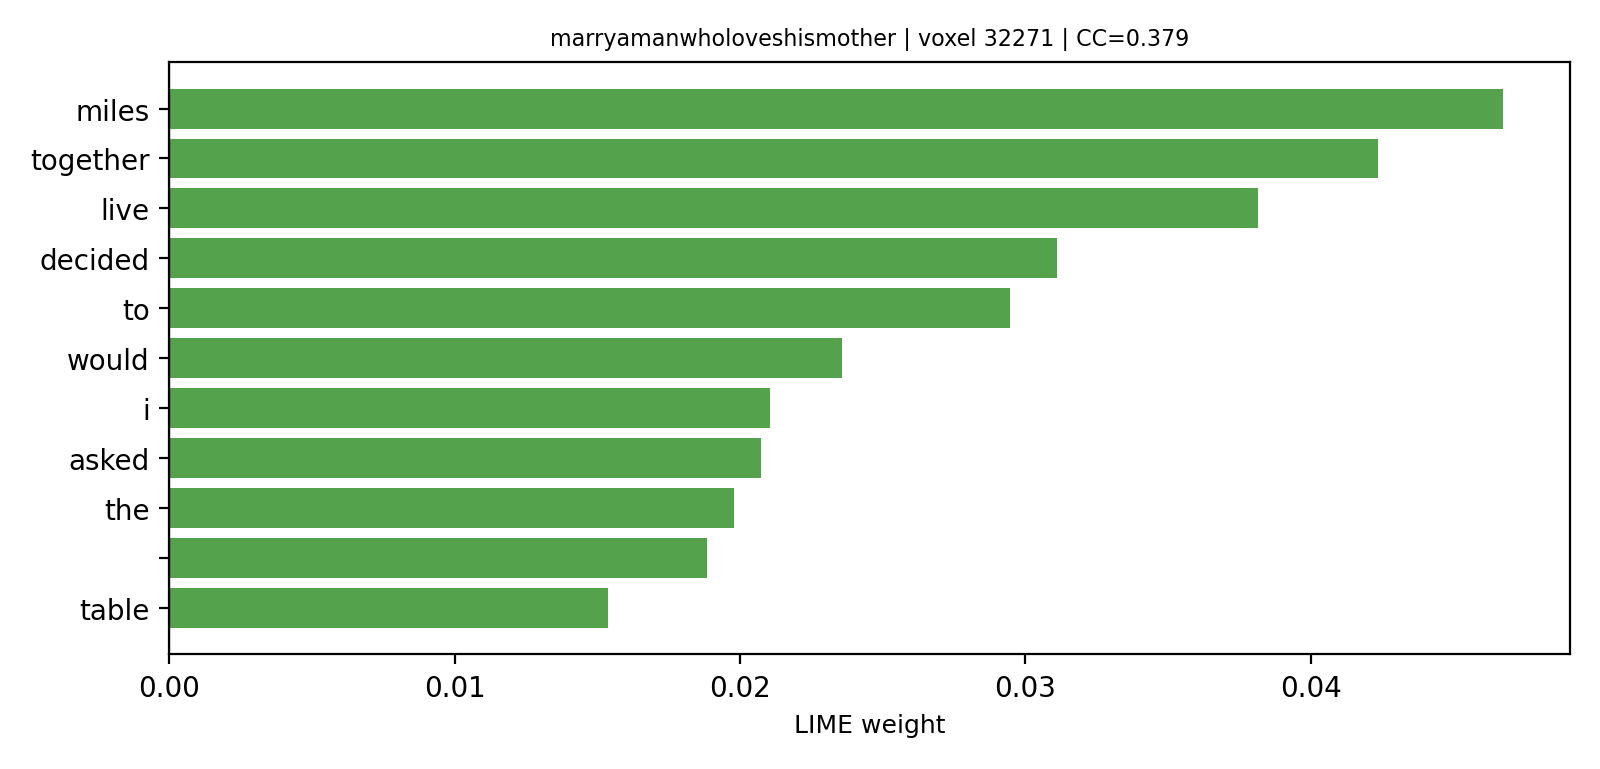
\includegraphics[width=\textwidth]{s2/finetuned_lora_mid4_mean/lime/marryamanwholoveshismother/voxel32271_rank2_lime.png}
    \caption{s2, rank-2 voxel (32271)}
  \end{subfigure}
  \hfill
  \begin{subfigure}[b]{0.48\textwidth}
    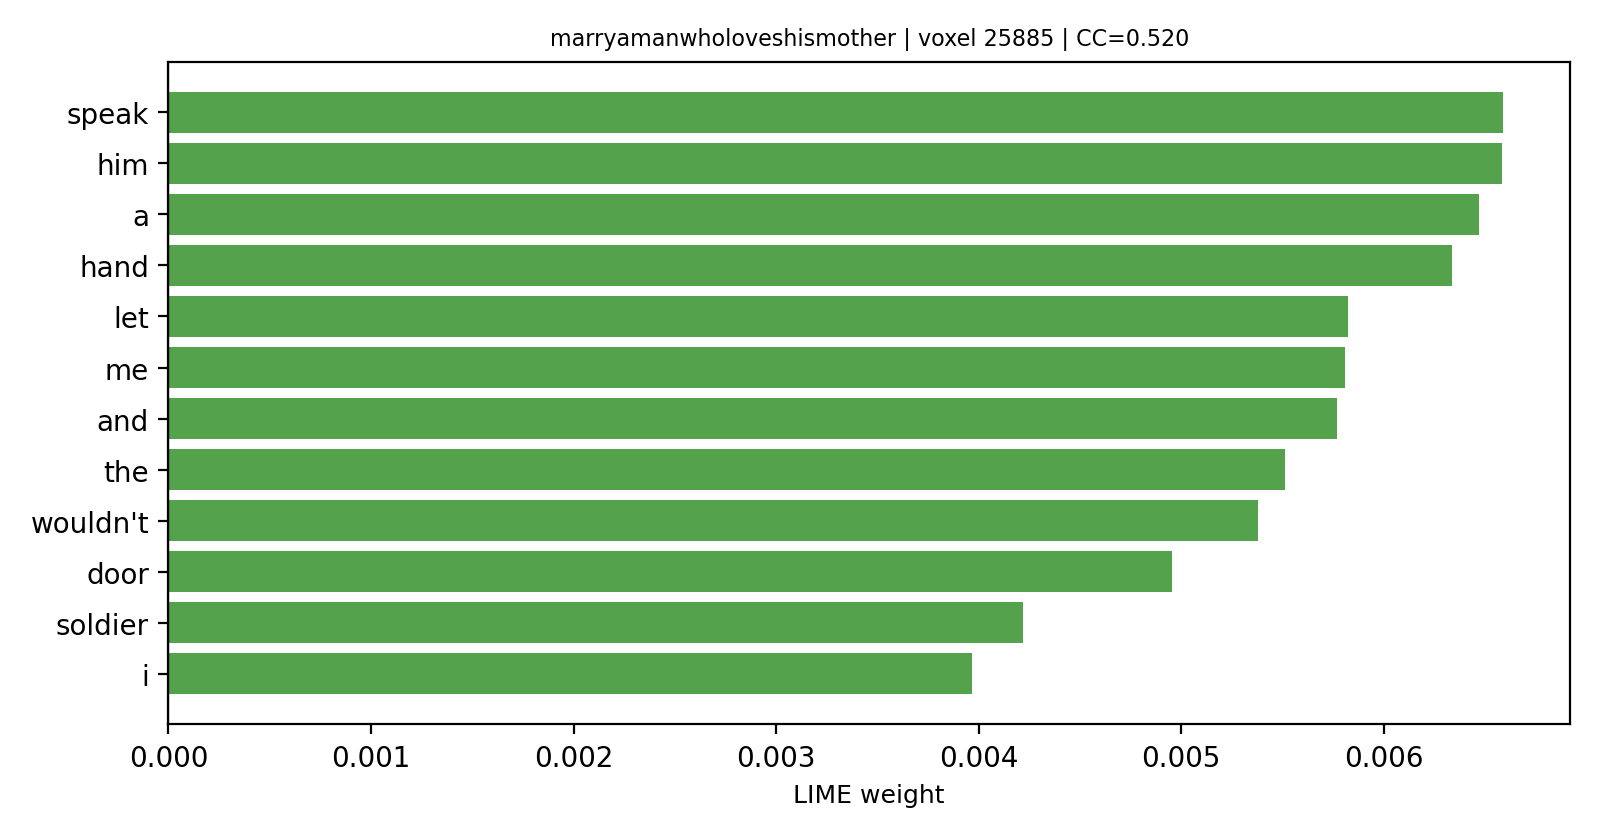
\includegraphics[width=\textwidth]{s3/finetuned_lora_mid4_mean/lime/marryamanwholoveshismother/voxel25885_rank2_lime.png}
    \caption{s3, rank-2 voxel (25885)}
  \end{subfigure}
  \caption{LIME word importances for \textit{Marry a Man Who Loves His Mother},
           rank-2 voxel per subject.}
  \label{fig:lime_marry_rank2}
\end{figure}

The response traces (Figure~\ref{fig:resp_marry}) place the highlighted window
in the latter portion of the story, where social negotiation between characters
reaches its narrative climax.  The model predictions closely follow the observed
signal in this region, again illustrating that prediction accuracy is
concentrated in semantically rich passages.

An inter-subject divergence emerges from the LIME attributions.  For s2,
high-importance words are relational verbs and adverbs describing co-habitation
and joint decisions: \texttt{miles}, \texttt{together}, \texttt{live},
\texttt{decided}, \texttt{asked}.  For s3, the leading terms are more concrete
physical-proximity and social-boundary words: \texttt{door}, \texttt{hand},
\texttt{came}, \texttt{let}, \texttt{soldier}, \texttt{wouldn't}.

Notably, the rank-1 and rank-2 voxels for each subject are immediate neighbours
in voxel index (s2: 32384 and 32271; s3: 25884 and 25885), yet their LIME
profiles diverge at a fine resolution while sharing the same social-proximity
theme.  This within-subject consistency is consistent with a smooth gradient of
semantic tuning in higher temporal cortex.


\subsection{Comparison of SHAP and LIME}

\subsubsection{Interpreted Results Layout}
SHAP and LIME answer related but distinct questions about the encoding model and
are best understood as complementary lenses rather than competing methods.
Table~\ref{tab:shap_vs_lime} summarises their key properties.

\begin{table}[ht]
  \centering
  \small
  \begin{tabular}{lll}
    \toprule
    & \textbf{SHAP} & \textbf{LIME} \\
    \midrule
    Scope        & Global across all test stories & Local to one story + one voxel \\
    Granularity  & BERT dim (768) + delay block   & Individual word token \\
    Attribution  & Closed-form: $\phi_j = X_{tj} w_j$ & Local linear surrogate (300 samples) \\
    Background   & Zero (z-scored features)       & Word masked to zero \\
    Time resolution & TR-level (2\,s windows)    & Word-level \\
    Output       & Feature importance across voxels & Word importance for peak window \\
    \bottomrule
  \end{tabular}
  \caption{Comparison of SHAP and LIME attribution methods as applied to the
           linear fMRI encoding model.}
  \label{tab:shap_vs_lime}
\end{table}

\subsubsection{Scope and Granularity}

SHAP operates globally: it aggregates over the entire test set and all 256
voxels to identify which BERT dimensions are systematically important across
stories and brain regions.  Its closed-form formula~(\ref{eq:shap}) requires no
sampling and is exact for linear models.  The cost is temporal resolution ---
because importance is averaged over all time steps, SHAP cannot resolve which
moments within a story drive the response.

LIME inverts this trade-off.  By constructing a local surrogate around the 5-TR
peak window of a single voxel's response, it achieves individual-word precision.
However, the 300-perturbation budget introduces sampling variance, the result is
specific to one story window and one voxel, and the local linear approximation
may not generalise to the broader response.

\subsubsection{Convergence on Key Content}

Despite their different scopes, SHAP and LIME converge on the same high-level
story content for both test stories.  For the Pluto story, SHAP identifies
TRs containing time-related vocabulary (``year'', ``old'', ``move'') as globally
important, and LIME independently assigns the highest word-level weights to
temporal mission markers (\texttt{july}, \texttt{fourth}, \texttt{working},
\texttt{long}) within the peak window.  For the relationship story, SHAP
highlights the dense spatial-description TR (``wooden'', ``chair'', ``propped''),
and LIME picks out the social-proximity words (\texttt{together},
\texttt{live}, \texttt{door}, \texttt{hand}) that dominate the narrative climax
window.

This cross-method agreement strengthens confidence that the identified content
reflects genuine neural selectivity rather than an artefact of either method's
design.

\subsubsection{Complementary Strengths}

The two methods provide distinct, non-redundant information:

\begin{itemize}
  \item \textbf{SHAP reveals latent BERT structure.}  By attributing importance
        to individual dimensions of the 768-dimensional BERT space, SHAP shows
        that brain-relevant semantic information is distributed across many
        dimensions (no single axis dominates) and is concentrated in early
        hemodynamic delays (delay block 1, 2\,s lag).  These findings hold
        globally across all stories and voxels and cannot be obtained from LIME,
        which operates on raw words rather than BERT features.

  \item \textbf{LIME reveals narrative-specific word salience.}  By linking
        response peaks to specific word tokens, LIME grounds the model's
        predictions in interpretable story content (mission dates, social
        actions) and enables comparison across subjects and adjacent voxels.
        SHAP word scores --- which assign the same value to all words in the
        same TR --- cannot distinguish between, say, \texttt{july} and
        \texttt{fourth} even though LIME shows them to have different
        contributions.

  \item \textbf{Response traces contextualise LIME windows.}  The predicted
        vs.\ observed traces (Figures~\ref{fig:resp_pluto}
        and~\ref{fig:resp_marry}) show that LIME's peak window corresponds to a
        moment of genuinely high predictive accuracy, validating that the local
        surrogate is explaining real signal rather than noise.  This cross-
        check is only possible because the encoding model provides continuous
        predictions that can be plotted against ground-truth BOLD.
\end{itemize}



\end{document}



\graphicspath{{results/stability/}}
\documentclass[letterpaper,12pt]{article}

\usepackage[margin=1in]{geometry}
\setlength\parindent{0pt}
\setlength{\parskip}{0.8em}

\usepackage{titlesec}
\titlespacing*{\section}{0pt}{0.5\baselineskip}{0.2\baselineskip}
\titlespacing*{\subsection}{0pt}{0.4\baselineskip}{0.1\baselineskip}

\usepackage{enumitem}
\setlist{nosep, topsep=2pt}

\usepackage{graphicx}
\graphicspath{{figures/stability/}}

\usepackage{subcaption}
\usepackage{booktabs}
\usepackage{amsmath}
\usepackage{amssymb}
\usepackage[hidelinks]{hyperref}

\title{Stability Analysis --- Lab 3\\
       \large Connecting Language to fMRI, Stat 214, Spring 2026\vspace{-1em}}
\date{}

\begin{document}
\maketitle


\section{Stability Analysis}

In the previous studies we have shown the variation of test results based on different choices of embedding
method, we will then assess the stability of out method based on whether they are robust to the choice
of subject.
In other words, does the ridge regression encoding model capture a real,
generalisable language-to-brain mapping that replicates across individuals,
or is it overfitting to idiosyncratic noise in one subject's data?
This is the central stability question, examined at four complementary levels
of granularity in this part
We apply this test to the \textbf{best-performing model} --- LoRA BERT
mid4$\star$ (layers 5--8 average, $d = 768$, delay-stacked to 3{,}072
features) --- on both subjects \textit{s2} (94{,}251 voxels) and \textit{s3}
(95{,}556 voxels).
Since a conservative test on a
weaker model would understate the replication that is actually achievable, we choose to only perform stability analysis on the best-performing model.



\subsection{Motivation}

If the encoding model captures a real, generalizable language-to-brain
mapping, the pattern of results should replicate across individuals even
though the two subjects differ physiologically and in brain coverage.
Direct voxel-index comparison is invalid: s2 has 94{,}251 voxels and s3
has 95{,}556, each in its own native space with no spatial registration.
We therefore assess replication at four complementary levels that do not
require a common voxel coordinate system, using the saved weight matrix
$W \in \mathbb{R}^{3072 \times n_\text{voxels}}$ from the LoRA mid4
ridge model.

\begin{enumerate}[label=(\arabic*)]
  \item \textbf{Story-level mean CC.}  For each subject, apply the fitted
        weights to the z-scored test embeddings, then compute the mean
        per-voxel Pearson~$r$ restricted to each of the 20 test stories.
        The resulting 20-dimensional profile is subject-count agnostic
        and directly comparable across subjects.
  \item \textbf{Per-story sorted bar chart.}  Visualise both profiles
        simultaneously, sorted by average CC, to identify which stories
        are universally easy or hard for the model to predict.
  \item \textbf{Voxelwise CC distributions.}  Compare the full
        per-voxel CC histograms for s2 and s3 to determine whether the
        s3 advantage is localised (a few high-CC voxels) or a uniform
        population-level shift.
\end{enumerate}

Additionally, we examine how the \textbf{cross-subject CC ratio}
($\overline{r}_{s3}/\overline{r}_{s2}$) varies across all eight embedding
methods to show that the replication pattern is not specific to LoRA mid4.

\subsection{Results}

\paragraph{Story-level replication.}
The headline summary is:

\begin{itemize}
  \item Story-level Pearson $r$ (s2 vs.\ s3, $n = 20$): $\mathbf{0.745}$
  \item s2 mean CC: $0.0374$, median $0.0330$;\quad
        s3 mean CC: $0.0512$, median $0.0432$
  \item s3 $>$ s2 in \textbf{17 of 20} test stories
  \item Top-1\% CC threshold: s2 $= 0.133$, s3 $= 0.180$
  \item Positive voxels: s2 $= 95.5\%$, s3 $= 97.8\%$
\end{itemize}


Figure~\ref{fig:check2_bars} (panel~B) sorts all 20 stories by average CC
and plots s2 and s3 side by side.  Three patterns stand out.
\textit{High for both subjects}:
\textit{onapproachtopluto} (s2 $= 0.075$, s3 $= 0.097$) and
\textit{fromboyhoodtofatherhood} (s2 $= 0.067$, s3 $= 0.098$) are
structurally rich, event-driven narratives whose contextual semantics the
fine-tuned BERT representations capture robustly.
\textit{marryamanwholoveshismother} (s2 $= 0.045$, s3 $= 0.065$) is
similarly well-predicted by both subjects.
\textit{Relatively lower for both}:
\textit{thatthingonmyarm} (s2 $= 0.019$, s3 $= 0.043$),
\textit{goingthelibertyway} (s2 $= 0.022$, s3 $= 0.058$), and
\textit{theadvancedbeginner} (s2 $= 0.020$, s3 $= 0.044$) rank lowest
for s2; notably these stories still produce meaningful CC under the best
model, whereas GloVe yielded near-zero predictions for the weakest stories.
\textit{Reversal stories} (s2 $>$ s3, marked $\star$):
only three stories reverse the typical ordering ---
\textit{reachingoutbetweenthebars} (s2 $= 0.060$, s3 $= 0.046$),
\textit{birthofanation} (s2 $= 0.036$, s3 $= 0.034$), and
\textit{canplanetearthfeedtenbillionpeoplepart1}
(s2 $= 0.028$, s3 $= 0.024$) --- consistent with individual variation
rather than a systematic pattern.

\paragraph{Voxelwise CC distributions.}
Figure~\ref{fig:check2_voxel} (panel~C) shows the full per-voxel CC
histograms for both subjects under the LoRA mid4 model.
Two features stand out compared to GloVe.
First, the distributions are strongly right-shifted: 95.5\% of s2 voxels
and 97.8\% of s3 voxels have positive CC, versus roughly 60--70\% under
GloVe.  The model predicts the direction of response correctly for almost
every voxel.
Second, the s3 distribution is again shifted uniformly rightward, with
the s3 mean (0.051) exceeding the s2 mean (0.037) across the entire
voxel population --- the advantage is not confined to a small elite of
top voxels.


\begin{center}
\begin{tabular}{lcc}
  \toprule
  Method & s2 mean CC & s3/s2 ratio \\
  \midrule
  BoW                  & 0.0069 & $1.99\times$ \\
  Word2Vec             & 0.0124 & $1.87\times$ \\
  GloVe                & 0.0128 & $1.72\times$ \\
  Vanilla BERT         & 0.0218 & $1.62\times$ \\
  Enhanced BERT        & 0.0349 & $1.41\times$ \\
  LoRA (last4/improved)& 0.0344 & $1.42\times$ \\
  LoRA (mid4$\star$)   & 0.0374 & $1.37\times$ \\
  \bottomrule
\end{tabular}
\end{center}

The shrinking ratio means that better embeddings not only raise absolute
CC but also \emph{close the gap between subjects}: richer semantic
representations recover signal that is present in both brains but
suppressed under weaker models.  This convergence is itself a replication
argument --- if the model were capturing idiosyncratic noise in one
subject, the inter-subject ratio would not change systematically with
embedding quality.



\begin{figure}[H]
  \centering
  
\includegraphics[width=\linewidth]{check2_mid4_B_story_bars}
  \caption{\textbf{Check 2 (panel B) --- Per-story encoding accuracy for
           both subjects (LoRA mid4$\star$), sorted by mean CC.}  Dashed
           lines mark each subject's global mean CC.  $\star$ = the three
           stories where s2 outperforms s3.  All stories produce positive
           mean CC under the best model; the ranking is highly consistent
           across subjects.}
  \label{fig:check2_bars}
\end{figure}

\begin{figure}[H]
  \centering
    
\includegraphics[width=0.8\linewidth]{check2_mid4_C_distributions}
    \caption{Full per-voxel CC distributions for both subjects (LoRA
             mid4$\star$).  95.5\% of s2 voxels and 97.8\% of s3 voxels
             are positive; s3 (red) is shifted uniformly rightward.
             Dashed lines = subject means; dotted lines = top-1\%
             thresholds.}
    \label{fig:check2_voxel}
\end{figure}


\end{document}


\section{Discussion}
In this study, we investigated human cortical processing of language by evaluating various text embedding models against fMRI responses in different regions of the human brain. Our results demonstrate a clear hierarchy in predictive power: contextualized language models (BERT) vastly outperform static semantic vectors including GloVe and Word2Vec, which in turn outperform non-semantic baseline Bag-ofWords. This progression underscores that contextual integration in embeddings are more likely applied in actual language representation in cortical processing rather than isolated processing of static lexical items.


The stark performance gap between static word vectors (GloVe, Word2Vec) and contextualized models (Base and Fine-tuned BERT) illustrates that contextual integration is essential human language comprehension. Static embeddings functioning with isolated lexical values assigns a fixed coordinate to a word regardless of its surrounding syntax or background story, whic is not fitting to represent the human brain actively that integrates temporal context, continuously updating its semantic representations based on previous discourse. The superior predictive correlation of BERT indicates that self-attention mechanism captures such dynamic integration more successfully, giving it a better performance in predicting BOLD signal fluctuations in higher-order language networks.


One revealing finding of our study is the layer phenomenon observed within the BERT architecture. The significant performance boost achieved by extracting representations from the middle layers (layers 5--8) rather than the final layers (layers 9--12) provides a critical window into how deep learning architectures diverge from biological networks. Instead of processing from basic acoustic/lexical features in early layers to complex syntactic and semantic structures in the middle, the highest layers, however, become hyper-specialized for the model's pre-training objective of word prediction, or in this case, Masked Language Modeling. Our results suggest that the generalized semantic structures formed in the middle layers align most naturally with human cortical processing, whereas the top-layer MLM representations represent an algorithmic artifact that does not seem to align with raw fMRI data.




Despite these insights, our approach is constrained by the reliance on a strictly linear mapping function of Ridge regression. While linear models are standard in fMRI encoding to prevent overfitting and ensure interpretability, they implicitly assume that the brain's semantic space is a direct linear projection of the Transformer's latent space. Future work should explore whether non-linear mappings can capture additional variance without sacrificing the interpretability provided by SHAP. Incorporating joint multimodal models that process both the raw audio waveform and the semantic text could decouple low-level auditory processing from high-level semantic integration, providing a more comprehensive model of naturalistic language comprehension.



\section{Conclusion}

This study successfully demonstrated that contextually integrated embedding models provide a vastly superior computational framework for modeling human cortical language processing compared to static and non-semantic baseline models. By mapping various text embeddings to fMRI BOLD responses using Ridge regression, we observed a clear progression in predictive accuracy: models that dynamically integrate temporal and syntactic context, such as Enhanced BERT, most successfully modeled the biological process of human language comprehension in the human brain. 

Our investigation into the internal architecture of embedding models yielded several insights. Specifically, the layer-wise performance disparity revealed that the middle layers of BERT align most robustly with generalized human semantic processing. Conversely, the highest layers exhibit a divergence from biological processing, likely due to overfitting of the word prediction objective. Furthermore, the plateau in predictive gains following LoRA fine-tuning on the podcast corpus suggests a near-optimal result for BERT models, while also implying that while foundational models already capture rich naturalistic representations, the MLM objective itself may not perfectly approximate human predictive coding.

Finally, the integration of feature attribution methods, namely SHAP and LIME, was instrumental in moving beyond black-box predictive metrics for our language modeling. By explicitly linking highly predicted voxels to semantically relevant stimulus words, we provided essential biological validation that our models successfully captured localized neural tuning curves rather than exploiting mathematical artifacts. Ultimately, this work highlights the immense potential of pairing modern Fine-Tuning methodologies with robust interpretability frameworks to investigate the cognitive architecture of language. 

\section*{Academic Honesty Statement}
\subsection{Statement}
The work in this report is our own and all the sources used are properly cited. Academic research honesty is important because science is built on truth.
\subsection{LLM Usage}


\subsubsection*{Coding}
\begin{itemize}
    \item Team member 1: I used Anthropic's Claude to understand better how to improve code, to suggest ways to "prettify" some of the visuals.
    \item Team member 2: I used Gemini to brainstorm possible ways of implementing models. I also used this model to polish my already-existing writings.
    \item Team member 3:  I used ChatGPT to clean the code, create documentation, and brainstorm the method in order to improve the performance.
    \item Team member 4:  I used Claude Code to modify the style of code, create documentation, and help me plot figures.
\end{itemize}

\subsubsection*{Writing}
\begin{itemize}
    \item Used to find grammatical errors and LaTeX formatting (e.g. tables).
\end{itemize}



\bibliographystyle{plain}
\bibliography{refs}
\bibitem{jain2018incorporating}
Jain, S., \& Huth, A. (2018).
Incorporating context into language encoding models for fMRI.
\textit{Advances in Neural Information Processing Systems}, 31.


\bibitem{hu2022lora}
Hu, E., et al. (2022). LoRA: Low-rank adaptation of large language models.
\textit{ICLR 2022}.

\bibitem{lundberg2017unified}
Lundberg, S. M., \& Lee, S.-I. (2017).
A unified approach to interpreting model predictions.
\textit{Advances in Neural Information Processing Systems}, 30.

\bibitem{ribeiro2016why}
Ribeiro, M. T., Singh, S., \& Guestrin, C. (2016).
"Why should I trust you?": Explaining the predictions of any classifier.
\textit{Proceedings of the 22nd ACM SIGKDD International Conference on Knowledge Discovery and Data Mining}.
\end{document}
